\section{Correction} \label{Corr}
\graphicspath{{images/corr}}

In this section, we will look at the different correction methods. we will start by presenting the different problems considered (Section \ref{Corr.problems}), then we will introduce the different correction methods (Section \ref{Corr.methods}), more specifically correction by addition, correction by multiplication and correction by multiplication on a so-called elevated problem. We will then continue by presenting some theoretical results on these different methods (Section \ref{Corr.theo_results}), and finish by presenting the numerical results obtained (Section \ref{Corr.results}).

\subsection{Presentation of different problems considered} \label{Corr.problems}

In this section, we present the different problems we will be considering in Section \ref{Corr.results}. We will consider the geometry of a circle in Section \ref{Corr.pb.circle} represented in Figure \ref{geom_circle} as well as the geometry of a square in Section \ref{Corr.pb.square} represented in Figure \ref{geom_square}. For the circle, we will consider a first analytic trigonometric solution, parameterized in such a way that the problem can be considered homogeneous. we will then consider a second problem for which no exact solution is known, and for which we will take an over-refined FEM solution as the reference solution. For the square, we will consider only an analytic trigonometric solution parameterized in such a way that the problem can be considered homogeneous.

\begin{minipage}{0.48\linewidth}
	\begin{figure}[H]
		\centering
		\includegraphics[width=0.6\linewidth]{"geom_circle.png"}
		\captionof{figure}{Representation of the first domain considered : the Circle.}
		\label{geom_circle}
	\end{figure} 
\end{minipage} $\qquad$
\begin{minipage}{0.48\linewidth}
	\begin{figure}[H]
		\centering
		\includegraphics[width=0.6\linewidth]{"geom_square.png"}
		\captionof{figure}{Representation of the second domain considered : the Square.}
		\label{geom_square}
	\end{figure} 
\end{minipage}

\begin{Rem}
	To generate meshes with FEM, we will consider a mesh comparable to $\phi$-FEM. To do this, we generate our $\phi$-FEM grid, which is simply the regular mesh of the $\mathcal{O}$ domain of $n_{vert}\times n_{vert}$ nodes. From this mesh we generate a FEM mesh whose largest element diameter $h_{FEM}$ is very close to the largest diameter associated with $\phi-FEM$, $h_{\phi-FEM}$ ($h_{FEM}\sim h_{\phi-FEM}$). Here, we have a representation of the meshes generated for FEM and $\phi$-FEM on the circle (Figure \ref{mesh_circle}) and on the square (Figure \ref{mesh_square}) with $n_{vert}=10$ vertices in each direction.
	
	\begin{minipage}{0.48\linewidth}
		\begin{figure}[H]
			\centering
			\includegraphics[width=\linewidth]{"mesh_circle.png"}
			\captionof{figure}{Representation of meshes for FEM and $\phi$-FEM on the Circle.}
			\label{mesh_circle}
		\end{figure} 
	\end{minipage} $\qquad$
	\begin{minipage}{0.48\linewidth}
		\begin{figure}[H]
			\centering
			\includegraphics[width=\linewidth]{"mesh_square.png"}
			\captionof{figure}{Representation of meshes for FEM and $\phi$-FEM on the Square.}
			\label{mesh_square}
		\end{figure} 
	\end{minipage}
\end{Rem}

\begin{Rem}
	Note that in the case where the problem is non-homogeneous, if we don't have a definition of the Dirichlet boundary condition, we can consider
	\begin{equation*}
	g(x,y)=u_{ex}(x,y)\times(1+\phi(x,y))
	\end{equation*}
	with $\phi$ the level-set function, null by definition on $\Gamma$.
\end{Rem}

\subsubsection{First domain : the Circle.} \label{Corr.pb.circle}

Here, we will consider the $\Omega$ domain to be the circle of radius $\sqrt{2}/4$ and center $(0.5,0.5)$.This domain is entirely included in the fictitious domain $O=[0,1]^2$ (Figure \ref{geom_circle}).

We will consider the level-set function $\phi$ defined by
\begin{equation*}
	\phi(x,y)=-1/8+(x-1/2)^2+(y-1/2)^2,
\end{equation*}
negative function inside the domain, null at the boundary and positive outside it
	
We will consider a first analytic trigonometric solution (Section \ref{Corr.pb.circle.1}), parameterized in such a way that the problem can be considered homogeneous and then consider a second problem (Section \ref{Corr.pb.circle.2}) for which no exact solution is known, and for which we'll take an over-refined FEM solution as the reference solution.

\paragraph{First problem} \label{Corr.pb.circle.1}

Here, we are interested in the Poisson problem with an analytical solution
\begin{equation*}
	u_{ex}(x,y)=S\times\sin\left(8\pi f\left((x-0.5)^2+(y-0.5)^2\right)+\varphi\right)
\end{equation*}
where $S\in[0,1]$ is the amplitude of the signal, $f\in\mathbb{N}$ can be associated with the "frequency" of the signal and $\varphi\in[0,1]$ the phase at the origin, represented in Figure \ref{sol_circle}.

Thus, the second associated member is defined by
\begin{align*}
	f(x,y)=256\pi^2 S f^2&\left((x-0.5)^2+(y-0.5)^2\right)\sin\left[8\pi f\left((x-0.5)^2+(y-0.5)^2\right) + \varphi\right] \\
	&- 32\pi S f\cos\left[8\pi f \left((x-0.5)^2+(y-0.5)^2\right) + \varphi\right]
\end{align*}
and represented in Figure \ref{f_circle}.

\begin{Rem}
	Note that for $\varphi=0$, the Dirichlet conditions considered are then homogeneous on the circle (i.e. $g=0$ on $\Gamma$).
\end{Rem}

\begin{minipage}{0.48\linewidth}
	\begin{figure}[H]
		\centering
		\includegraphics[width=\linewidth]{"sol_circle.png"}
		\captionof{figure}{Representation of the solution $u_{ex}$ on the Circle with $S=0.5$ and $f=1$ (with $p=0$ and $p=1$).}
		\label{sol_circle}
	\end{figure} 
\end{minipage} $\qquad$
\begin{minipage}{0.48\linewidth}
	\begin{figure}[H]
		\centering
		\includegraphics[width=\linewidth]{"f_circle.png"}
		\captionof{figure}{Representation of the term $f$ on the Circle with $S=0.5$ and $f=1$ (with $p=0$ and $p=1$).}
		\label{f_circle}
	\end{figure} 
\end{minipage}

\paragraph{$f$ Gaussian} \label{Corr.pb.circle.2}

In the case considered here, no analytical solution is known. We consider the source term $f$ to be a Gaussian defined by
\begin{equation*}
	f(x,y) = \exp\left(-\frac{(x-\mu_0)^2 + (y-\mu_1)^2}{2\sigma^2}\right)\,,
\end{equation*} 
with $\sigma \sim \mathcal{U}([0.1,0.6])$ and $\mu_0, \mu_1 \sim \mathcal{U}([0.5-\sqrt{2}/4, 0.5+\sqrt{2}/4])$ with the condition $\phi(\mu_0, \mu_1) < -0.05$ and represented in Figure \ref{f_circle_gaussian}

Since we don't have an exact solution, we will consider a so-called reference solution, denoted $u_{ref}$. This reference solution is defined as an over-refined $\mathbb{P}^1$ solution obtained by the standard FEM method (with $h_{ref}\approx 0.006$). It is to this reference solution that we can compare the solutions obtained by the correction methods or by the FNO.

\begin{Rem}
	For this problem, we choose to consider only the homogeneous case, i.e. we take $g=0$ on $\Gamma$.
\end{Rem}

\begin{figure}[H]
	\centering
	\includegraphics[width=0.3\linewidth]{"f_circle_gaussian.png"}
	\captionof{figure}{Representation of the term $f$ on the Circle with $(\mu_0,\mu_1)=(0.5,0.5)$ and $\sigma=0.3$.}
	\label{f_circle_gaussian}
\end{figure} 

\subsubsection{Second domain : the Square.} \label{Corr.pb.square}

Here, we will consider the $\Omega$ domain to be the unit square $\Omega=[0,1]^2$. This domain is entirely included in the fictitious domain $O=[-0.5,1.5]^2$ (Figure \ref{geom_square}).

In this case, we will consider two level-set functions. The first function $\phi$, defined by
\begin{equation*}
	\phi(x,y)=x(1-x)y(1-y),
\end{equation*}
will be used when solving the weak problem. However, it cannot be used to construct our cell and face sets, because it is not only negative in the $\Omega$ domain (Figure \ref{levelset_square}).

\begin{figure}[H]
	\centering
	\includegraphics[width=0.3\linewidth]{"levelset_square.png"}
	\captionof{figure}{Representation of $\phi(x,y)<0$.}
	\label{levelset_square}
\end{figure} 

To construct the sets of cells and faces needed to perform the $\phi$-FEM method, we will consider a second function, denoted $\phi_C$ and defined by
\begin{equation*}
	\phi_C(x,y)=\max(|x-0.5|,|y-0.5|)-0.5,
\end{equation*}
which is indeed negative inside the domain, zero at the boundary and positive outside, but which does not sufficiently satisfy the regularity conditions necessary for $\phi$-FEM.

We will consider only an analytic trigonometric solution parameterized in such a way that the problem can be considered homogeneous.

\paragraph{Problem} \label{Corr.pb.square.1}

Here, we are interested in the Poisson problem with as analytical solution
\begin{equation*}
	u_{ex}(x,y)=S\times\sin\left(2\pi fx+\varphi\right)\times\sin\left(2\pi fy+\varphi\right)
\end{equation*}
where $S\in[0,1]$ is the amplitude of the signal, $f\in\mathbb{N}$ can be associated with the "frequency" of the signal and $\varphi\in[0,1]$ the phase at the origin.

Thus, the associated second member is defined by
\begin{equation*}
	f(x,y)=8\pi^2 Sf^2\sin\left(2\pi fx + \varphi\right)\sin\left(2\pi fy + \varphi\right)
\end{equation*}

\begin{Rem}
	It should be noted that as for the circle for $\varphi=0$, the Dirichlet conditions considered are then homogeneous on the square (i.e. $g=0$ on $\Gamma$).
\end{Rem}

\begin{minipage}{0.48\linewidth}
	\begin{figure}[H]
		\centering
		\includegraphics[width=\linewidth]{"sol_square.png"}
		\captionof{figure}{Representation of the solution $u_{ex}$ on the Circle with $S=0.5$ and $f=1$ (with $p=0$ and $p=1$).}
		\label{sol_square}
	\end{figure} 
\end{minipage} $\qquad$
\begin{minipage}{0.48\linewidth}
	\begin{figure}[H]
		\centering
		\includegraphics[width=\linewidth]{"f_square.png"}
		\captionof{figure}{Representation of the term $f$ on the Circle with $S=0.5$ and $f=1$ (with $p=0$ and $p=1$).}
		\label{f_square}
	\end{figure} 
\end{minipage}

\subsection{Presentation of the different correction methods considered} \label{Corr.methods}

Here we are given $\tilde{\phi}$ an "initial" solution to the problem under consideration, i.e. a solution that has not yet been corrected. This may be a perturbed analytic solution, a $\phi$-FEM solution, or a solution predicted by a neural network (such as an FNO, a Multi-perceptron network or PINNs, for example). The aim is to inject this solution into a new problem in order to improve the accuracy of the solution. To achieve this, we consider 3 types of correction: correction by addition (Section \ref{Corr.method.add}), correction by multiplication (Section \ref{Corr.method.mult}) and correction by multiplication on an elevated problem (Section \ref{Corr.method.mult_reh}).

\begin{Rem}
	In what follows, we assume that $\tilde{\phi}$ already has the right conditions at the boundary, i.e. $\tilde{\phi}=g$ on $\Gamma$.
\end{Rem}

\subsubsection{Correction by adding} \label{Corr.method.add}

In this first method, we will try to approximate the solution obtained $\tilde{\phi}$ to the exact solution by completing the difference between the two, which is what we will call correction by adding. To do this, we will consider
\begin{equation*}
	\tilde{u}=\tilde{\phi}+\tilde{C}
\end{equation*}
and we want to find $\tilde{C}: \Omega \rightarrow \mathbb{R}^d$ solution to the problem
\begin{equation*}
	\left\{\begin{aligned}
		-\Delta \tilde{u}&=f, \; &&\text{on } \Omega, \\
		\tilde{u}&=g, \; &&\text{in } \Gamma.
	\end{aligned}\right.
\end{equation*}
\begin{Rem}
	Note that this problem is in fact equivalent to the initial problem. We only hope that the approximate solution $\tilde{u}$ obtained is more accurate than the approximate solution $u$ obtained by solving the initial problem.
\end{Rem}
Rewriting the problem, we seek to find $\tilde{C}: \Omega \rightarrow \mathbb{R}^d$ solution to the problem
\begin{equation*}
\left\{\begin{aligned}
	-\Delta \tilde{C}&=\tilde{f}, \; &&\text{on } \Omega, \\
	\tilde{C}&=0, \; &&\text{in } \Gamma.
\end{aligned}\right. %\tag{$\mathcal{C}_{+}$}
\end{equation*}
with $\tilde{f}=f+\Delta\tilde{\phi}$.

Thus for the standard FEM method, the weak formulation will be given by
\begin{equation*}
	\int_\Omega \nabla\tilde{C}\cdot\nabla v=\int_\Omega \tilde{f}v
\end{equation*}
where the homogeneous Dirichlet conditions can be strongly imposed by classical methods (penalization, elimination...).

For the $\phi$-FEM method, we look for $C$ such that $\tilde{C}=\phi C$ and the weak formulation (associated with a homogeneous problem because $\tilde{C}=0$ on $\Gamma$) is given by
\begin{equation*}
	\int_{\Omega_h} \nabla (\phi C) \cdot \nabla (\phi v) - \int_{\partial\Omega_h} \frac{\partial}{\partial n}(\phi C)\phi v+G_h(w,v)=\int_{\Omega_h} \tilde{f} \phi v + G_h^{rhs}(v)
\end{equation*}
with
\begin{equation*}
	G_h(C,v)=\sigma h\sum_{E\in\mathcal{F}_h^\Gamma} \int_E \left[\frac{\partial}{\partial n}(\phi C)\right] \left[\frac{\partial}{\partial n}(\phi v)\right]+\sigma h^2\sum_{T\in\mathcal{T}_h^\Gamma} \int_{T} \Delta(\phi C)\Delta(\phi v)
\end{equation*}
and
\begin{equation*}
	G_h^{rhs}(v)=-\sigma h^2\sum_{T\in\mathcal{T}_h^\Gamma} \int_{T} \tilde{f} \Delta(\phi v).
\end{equation*}

In the non-homogeneous case, the formulation is the same, as the correction problem stays homogeneous ($\tilde{C}=0$ on $\Gamma$).

\begin{Rem}
	In practice, it may be useful to integrate by parts (IPP) the term containing $\Delta \tilde{\phi}$ (implicitly included in $\tilde{f}$).
	
	So for FEM, as $v\in H_0^1(\Omega)$, we have
	\begin{equation*}
		\int_\Omega \tilde{f}v=\int_\Omega fv+\int_\Omega \Delta\tilde{\phi}v=\int_\Omega fv-\int_\Omega \nabla\tilde{\phi}\cdot\nabla v.
	\end{equation*}
	For $\phi$-FEM, we have
	\begin{equation*}
		\int_{\Omega_h} \tilde{f} \phi v=\int_{\Omega_h} f \phi v+\int_{\Omega_h} \Delta\tilde{\phi} \phi v=\int_{\Omega_h} f \phi v-\int_{\Omega_h} \nabla\tilde{\phi}\cdot\nabla(\phi v)+\int_{\partial\Omega_h} \frac{\partial\tilde{\phi}}{\partial n}\phi v.
	\end{equation*}
\end{Rem}

\subsubsection{Correction by multiplying} \label{Corr.method.mult}

In this second method, we try to approach the exact solution in a different way. In fact, we want to bring the factor between the $\tilde{\phi}$ solution and the solution of the corrected problem closer to 1. In other words, by considering 
\begin{equation*}
	\tilde{u}=\tilde{\phi}C,
\end{equation*}
we try to bring $C=\frac{\tilde{u}}{\tilde{\phi}}$ closer to 1 (for $\tilde{\phi}\ne 0$). This type of correction is called correction by multiplying.

So we're looking for $C: \Omega \rightarrow \mathbb{R}^d$ solution to the problem
\begin{equation*}
	\left\{\begin{aligned}
		&-\Delta (\tilde{\phi}C)=f, \; &&\text{on } \Omega, \\
		&C=1, \; &&\text{on } \; \Gamma.
	\end{aligned}\right. %\tag{$\mathcal{C}_\times$}
\end{equation*}

\begin{Rem}
	In the same way as for correction by adding, we note that this problem is equivalent to the initial problem.
\end{Rem}

So for the standard FEM method, the weak formulation will be given by
\begin{equation*}
	\int_\Omega \nabla (\tilde{\phi}C)\cdot\nabla (\tilde{\phi}v)=\int_\Omega f\tilde{\phi}v
\end{equation*}
where homogeneous or non-homogeneous Dirichlet conditions can be strongly imposed by classical methods (penalization, elimination...).

For the $\phi$-FEM method, the weak formulation for the homogeneous problem is given by
\begin{equation*}
	\int_{\Omega_h} \nabla (\tilde{\phi} C) \cdot \nabla (\tilde{\phi} v) - \int_{\partial\Omega_h} \frac{\partial}{\partial n}(\tilde{\phi} C)\tilde{\phi} v+G_h(w,v)=\int_{\Omega_h} f \tilde{\phi} v + G_h^{rhs}(v)
\end{equation*}
with
\begin{equation*}
	G_h(C,v)=\sigma h\sum_{E\in\mathcal{F}_h^\Gamma} \int_E \left[\frac{\partial}{\partial n}(\tilde{\phi} C)\right] \left[\frac{\partial}{\partial n}(\tilde{\phi} v)\right]+\sigma h^2\sum_{T\in\mathcal{T}_h^\Gamma} \int_{T} \Delta(\tilde{\phi} C)\Delta(\tilde{\phi} v)
\end{equation*}
and
\begin{equation*}
	G_h^{rhs}(v)=-\sigma h^2\sum_{T\in\mathcal{T}_h^\Gamma} \int_{T} f \Delta(\tilde{\phi} v).
\end{equation*}

In the non-homogeneous case, it is important to impose the boundary conditions either by the direct method or by the dual method presented in Section \ref{FEMs.PhiFEM.details.nh}.

\subsubsection{Correction by multiplying on an elevated problem} \label{Corr.method.mult_reh}

We now introduce a third correction method, which we will call correction by multiplying on an elevated problem. This method is in fact very similar to the previous one (correction by multiplying), except that we are no longer trying to correct the same problem.

The initial modified problem, which we now consider, consists in finding $u : \Omega \rightarrow \mathbb{R}^d$ such that
\begin{equation*}
	\left\{
	\begin{aligned}
		-\Delta \hat{u} = f, \; &&\text{in } \; \Omega, \\
		\hat{u}=g+m, \; &&\text{on } \; \Gamma,
	\end{aligned}
	\right. %\tag{$\mathcal{P}^\mathcal{M}$}
\end{equation*}
with $\hat{u}=u+m$ and $m$ a constant.

We then apply the same multiplication correction method, but this time on the modified problem, which has been elevated by a constant $m$. We then consider
\begin{equation*}
	\tilde{u}=\hat{\phi}C
\end{equation*}
with 
\begin{equation*}
	\hat{\phi}=\tilde{\phi}+m
\end{equation*}
and so we look for $C: \Omega \rightarrow \mathbb{R}^d$ solution to the problem
\begin{equation*}
	\label{eq.corr.pbc_mult_reh}
	\left\{\begin{aligned}
		&-\Delta (\hat{\phi}C)=f, \; &&\text{in } \; \Omega, \\
		&C=1, \; &&\text{on } \; \Gamma.
	\end{aligned}\right. %\tag{$\mathcal{C}_\times^\mathcal{M}$}
\end{equation*}

So for the standard FEM method, the weak formulation will be given by
\begin{equation*}
	\int_\Omega \nabla (\hat{\phi}C)\cdot\nabla (\hat{\phi}v)=\int_\Omega f\hat{\phi}v
\end{equation*}
where homogeneous or non-homogeneous Dirichlet conditions can be strongly imposed by classical methods (penalization, elimination...)

For the $\phi$-FEM method, the weak formulation for the homogeneous problem is given by
\begin{equation*}
	\int_{\Omega_h} \nabla (\hat{\phi} C) \cdot \nabla (\hat{\phi} v) - \int_{\partial\Omega_h} \frac{\partial}{\partial n}(\hat{\phi} C)\hat{\phi} v+G_h(w,v)=\int_{\Omega_h} f \hat{\phi} v + G_h^{rhs}(v)
\end{equation*}
with
\begin{equation*}
	G_h(C,v)=\sigma h\sum_{E\in\mathcal{F}_h^\Gamma} \int_E \left[\frac{\partial}{\partial n}(\hat{\phi} C)\right] \left[\frac{\partial}{\partial n}(\hat{\phi} v)\right]+\sigma h^2\sum_{T\in\mathcal{T}_h^\Gamma} \int_{T} \Delta(\hat{\phi} C)\Delta(\hat{\phi} v)
\end{equation*}
and
\begin{equation*}
	G_h^{rhs}(v)=-\sigma h^2\sum_{T\in\mathcal{T}_h^\Gamma} \int_{T} f \Delta(\hat{\phi} v).
\end{equation*}

In the case of this correction, whether the problem is homogeneous or non-homogeneous, the correction problem is non-homogeneous (for $m\ne 0$), so it is important to impose the boundary conditions either by the direct method, or by the dual method presented in Section \ref{FEMs.PhiFEM.details.nh}.

\begin{Rem}
	Note that if the problem is sufficiently elevated for its solution to be strictly positive, the operation of bringing $C=\frac{\tilde{u}}{\hat{\phi}}$ closer to 1 doesn't pose any problem (since in this case $\hat{\phi}\ne 0$). Moreover, we can easily return to the original problem by subtracting $m$ from $\tilde{u}$.
\end{Rem}

\subsection{Theoretical results} \label{Corr.theo_results}

The aim of this section is to present some interesting theoretical results. We begin by presenting the interest of elevating the problem in Section \ref{Corr.theo_results.reh}. We will then present an interesting result for standard FEM in Section \ref{Corr.theo_results.comp_add_reh}. In fact, we'll show that the solution obtained by the multiplication correction on the elevated problem converges to the solution obtained by the addition correction when $m$ tends to infinity. Finally, we will demonstrate the estimation error of the correction on the elevated problem in Section \ref{Corr.theo_results.error_reh}.

\subsubsection{Interest of elevating the problem} \label{Corr.theo_results.reh}

The aim of this section is to explain the interest in elevating the problem in the case of the multiplication correction presented in Section \ref{Corr.method.mult_reh} with a $\mathbb{P}^1$ solution. Only the standard FEM method is considered here. For this purpose, we will consider a so-called disturbed solution, i.e. one that is close to the exact solution. We assume we have an analytical solution to the problem, denoted $u_{ex}$, to which we will apply a perturbation, denoted $P$. We then define
\begin{equation*}
	\tilde{\phi}(x,y) = u(x,y)+\epsilon P(x,y)
\end{equation*}
with $P$ the perturbation (such that $P=0$ on $\Gamma$) and $\epsilon$ small.

We pose
\begin{equation*}
	\hat{\phi}=\tilde{\phi}+m
\end{equation*}
with $m$ a constant, and consider the multiplication correction on a elevated problem, defined in Section \ref{Corr.method.mult_reh} by the problem
\begin{equation*}
	\left\{\begin{aligned}
		&-\Delta (\hat{\phi}C)=f, \; &&\text{in } \; \Omega, \\
		&\hat{u}=g+m, \; &&\text{on } \; \Gamma.
	\end{aligned}\right.
\end{equation*}
with $\hat{u}=\hat{\phi}C$.

In Section \ref{Corr.theo_results.error_reh}, we will prove the following inequality in the context of this problem

\begin{equation*}
	\left|\left|\hat{u_{ex}}-\hat{u_h}\right|\right|_0\le ch^{k+1}||\hat{\phi}||_\infty\left|C\right|_{k+1,\Omega}
\end{equation*}

with $c$ a constant, $\hat{u_{ex}}=u_{ex}+m$ and $C=\frac{u_{ex}+m}{\hat{\phi}}$.

For $k=1$, we then have
\begin{equation*}
	|C|_{2,\Omega}=\left|\frac{u_{ex}+m}{\hat{\phi}}\right|_{2,\Omega}=\left|\left|\left(\frac{u_{ex}+m}{\hat{\phi}}\right)''\right|\right|_{0,\Omega}=\epsilon\left|\left|\left(\frac{P}{\hat{\phi}}\right)''\right|\right|_{0,\Omega}=\epsilon\left|\left|\left(\frac{P}{\tilde{\phi}+m}\right)''\right|\right|_{0,\Omega}
\end{equation*}
with
\begin{align*}
	\left(\frac{P}{\tilde{\phi}+m}\right)''&=\frac{P''(\tilde{\phi}+m)-P\tilde{\phi}''}{(\tilde{\phi}+m)^2}+\frac{2(P\tilde{\phi}'-P'(\tilde{\phi}+m))\tilde{\phi}'}{(\tilde{\phi}+m)^3} \\
	&=\frac{P''\tilde{\phi}-P\tilde{\phi}''}{(\tilde{\phi}+m)^2}+\frac{2(P\tilde{\phi}'-P'\tilde{\phi})\tilde{\phi}'}{(\tilde{\phi}+m)^3}+    \frac{mP''}{(\tilde{\phi}+m)^2}-\frac{2mP'\tilde{\phi}'}{(\tilde{\phi}+m)^3}
\end{align*}

As 
\begin{equation*}
	\left|\left|\left(\frac{P}{\tilde{\phi}+m}\right)''\right|\right|_{0,\Omega}=\left|\left|\left(\frac{P}{m\left(1+\frac{\tilde{\phi}}{m}\right)}\right)''\right|\right|_{0,\Omega}=\frac{1}{m}\left|\left|\left(\frac{P}{1+\frac{\tilde{\phi}}{m}}\right)''\right|\right|_{0,\Omega}
\end{equation*}
and 
\begin{align*}
	\left(\frac{P}{1+\frac{\tilde{\phi}}{m}}\right)''=m\left(\frac{P}{\hat{\phi}}\right)''&=\frac{m(P''\tilde{\phi}-P\tilde{\phi}'')}{(\tilde{\phi}+m)^2}+\frac{2m(P\tilde{\phi}'-P'\tilde{\phi})\tilde{\phi}'}{(\tilde{\phi}+m)^3}+    \frac{m^2P''}{(\tilde{\phi}+m)^2}-\frac{2m^2P'\tilde{\phi}'}{(\tilde{\phi}+m)^3} \\
	&=\frac{m(P''\tilde{\phi}-P\tilde{\phi}'')}{m^2\left(1+\frac{\tilde{\phi}}{m}\right)^2}+\frac{2m(P\tilde{\phi}'-P'\tilde{\phi})\tilde{\phi}'}{m^3\left(1+\frac{\tilde{\phi}}{m}\right)^3}+    \frac{m^2P''}{m^2\left(1+\frac{\tilde{\phi}}{m}\right)^2}-\frac{2m^2P'\tilde{\phi}'}{m^3\left(1+\frac{\tilde{\phi}}{m}\right)^3} \\
	&=\frac{P''\tilde{\phi}-P\tilde{\phi}''}{m\left(1+\frac{\tilde{\phi}}{m}\right)^2}+\frac{2(P\tilde{\phi}'-P'\tilde{\phi})\tilde{\phi}'}{m^2\left(1+\frac{\tilde{\phi}}{m}\right)^3}+    \frac{P''}{\left(1+\frac{\tilde{\phi}}{m}\right)^2}-\frac{2P'\tilde{\phi}'}{m\left(1+\frac{\tilde{\phi}}{m}\right)^3} \\
\end{align*}
then, for $m$ sufficiently large :
\begin{equation*}
	\left|\left|\left(\frac{P}{1+\frac{\tilde{\phi}}{m}}\right)''\right|\right|_{0,\Omega}\sim\left|\left|P''\right|\right|_{0,\Omega}
\end{equation*}

Finally, for $m$ sufficiently large, we have $||\hat{\phi}||_\infty\sim m$ and thus
\begin{equation*}
	\left|\left|\frac{u_{ex}+m}{\hat{\phi}}-C_h\right|\right|_{0,\Omega}\le ch^{k+1}\epsilon\left|\left|P''\right|\right|_{0,\Omega}
\end{equation*}

We deduce that when $m$ is big, the error no longer depends on the solution but only on the perturbation $P$. These results were obtained numerically and are presented in Section \ref{Corr.results.disturbed}.

However, when $m$ is small, we can see that the error is dominated by the first derivatives and second derivatives of the disturbed solution $\tilde{\phi}$.

\begin{Rem}
	In addition, raising the problem can be extremely efficient when the solution cancels out on the domain. However, note that in the case of the addition correction presented in Section \ref{Corr.method.add}, elevated the problem is of no interest.
\end{Rem}

\subsubsection{Comparison of correction methods} \label{Corr.theo_results.comp_add_reh}

Here, we compare 2 methods, the addition correction method defined in Section \ref{Corr.method.add} and the multiplication correction method on a elevated problem defined in Section \ref{Corr.method.mult_reh}. In fact, we will show that when m tends to infinity, the solution of the multiplication correction on a elevated problem converges to the solution of the addition correction.

\textbf{Correction by adding :}

Let's start by looking at the form of the solution in the case of correction by addition. The decomposition of $u_h$ on the $(\varphi_1,\dots,\varphi_{N_h})$ basis of $V_h$ is written as follows for this problem

\begin{equation}
	u_h=C_h+\tilde{\phi}(x)=\left(\sum_{i=1}^{N_h}C_i\varphi_i\right)+\tilde{\phi}(x) \label{decomp_pbc2}
\end{equation}

We have 
\begin{equation}
	C_i=u_{ex}(x_i)-\tilde{\phi}(x_i) \label{C_i_2}
\end{equation}
with
\begin{equation}
	u_{ex}(x_i)=\tilde{\phi}(x_i)-\epsilon P(x_i) \label{u_x_i_2}
\end{equation}
With the 2 previous relations, we can develop \ref{decomp_pbc2} :
\begin{align*}
	u_h&=\tilde{\phi}(x)+\sum_{i=1}^{N_h}C_i\varphi_i \\
	&=\tilde{\phi}(x)+\sum_{i=1}^{N_h}(u(x_i)-\tilde{\phi}(x_i))\varphi_i \quad \text{by \ref{C_i_2}} \\
	&=\tilde{\phi}(x)+\sum_{i=1}^{N_h}(\tilde{\phi}(x_i)-\epsilon P(x_i)-\tilde{\phi}(x_i))\varphi_i \quad \text{by \ref{u_x_i_2}} \\
	u_h&=\tilde{\phi}(x)-\epsilon\sum_{i=1}^{N_h} P(x_i)\varphi_i \numberthis \label{result2}
\end{align*}

\textbf{Correction by multiplying on an elevated problem :}

We are now interested in the form of the solution in the case of multiplication correction on a elevated problem. The decomposition of $\hat{u_h}$ on the $(\varphi_1,\dots,\varphi_{N_h})$ basis of $V_h$ is written as follows for this problem

\begin{equation}
	\hat{u_h}=C_h\hat{\phi}=\left(\sum_{i=1}^{N_h}C_i\varphi_i\right)\hat{\phi}(x) \label{decomp_pbc1}
\end{equation}

We have 
\begin{equation}
	C_i=\frac{u(x_i)+m}{\hat{\phi}(x_i)}=\frac{u(x_i)+m}{\tilde{\phi}(x_i)+m} \label{C_i}
\end{equation}
with
\begin{equation}
	u(x_i)=\tilde{\phi}(x_i)-\epsilon P(x_i) \label{u_x_i}
\end{equation}
and
\begin{equation}
	\tilde{\phi}(x)=\tilde{\phi}(x_i)+(x-x_i)\tilde{\phi}'(x_i). \label{phi_tilde_x}
\end{equation}
Moreover, we have 
\begin{equation}
	\sum_{i=1}^{N_h}\varphi_i=1 \label{sum_base}
\end{equation}
With the 4 previous relations, we can develop \ref{decomp_pbc1} :
\begin{align*}
	\hat{u_h}&=\left(\sum_{i=1}^{N_h}C_i\varphi_i\right)\hat{\phi}(x) \\
	&=\left(\sum_{i=1}^{N_h}\frac{u(x_i)+m}{\tilde{\phi}(x_i)+m}\varphi_i\right)\hat{\phi}(x) \quad \text{by \ref{C_i}} \\
	&=\left(\sum_{i=1}^{N_h}\frac{\tilde{\phi}(x_i)+m-\epsilon P(x_i)}{\tilde{\phi}(x_i)+m}\varphi_i\right)\hat{\phi}(x) \quad \text{by \ref{u_x_i}} \\
	&=\sum_{i=1}^{N_h}\left(1-\epsilon\frac{ P(x_i)}{\tilde{\phi}(x_i)+m}\right)\varphi_i\hat{\phi}(x) \\
	&=\left(\sum_{i=1}^{N_h}\varphi_i\right)\hat{\phi}(x)-\epsilon\sum_{i=1}^{N_h}P(x_i)\frac{\hat{\phi}(x)}{\tilde{\phi}(x_i)+m}\varphi_i \\
	&=\hat{\phi}(x)-\epsilon\sum_{i=1}^{N_h}P(x_i)\frac{\tilde{\phi}(x_i)+m+(x-x_i)\tilde{\phi}'(x_i)}{\tilde{\phi}(x_i)+m}\varphi_i \quad \text{by \ref{phi_tilde_x} et \ref{sum_base}} \\
	&=\hat{\phi}(x)-\epsilon\sum_{i=1}^{N_h}P(x_i)\left(1+\frac{(x-x_i)\tilde{\phi}'(x_i)}{\tilde{\phi}(x_i)+m}\right)\varphi_i \\
	&=\tilde{\phi}(x)+m-\epsilon\sum_{i=1}^{N_h}P(x_i)\left(1+\frac{(x-x_i)\tilde{\phi}'(x_i)}{\tilde{\phi}(x_i)+m}\right)\varphi_i \\
\end{align*}

Thus
\begin{equation*}
	u_h=\hat{u_h}-m=\tilde{\phi}(x)-\epsilon\sum_{i=1}^{N_h}P(x_i)\left(1+\frac{(x-x_i)\tilde{\phi}'(x_i)}{\tilde{\phi}(x_i)+m}\right)\varphi_i
\end{equation*}
and finally
\begin{equation}
	u_h\xrightarrow[m\to\infty]{} \tilde{\phi}(x)-\epsilon\sum_{i=1}^{N_h}P(x_i)\varphi_i \label{result1}
\end{equation}

So by \ref{result2} and \ref{result1}, it would seem that the 2 proposed methods are equivalent (taking $m$ to be large).

\begin{Rem}
	Taking $m=0$, we return to the case of correction by multiplication defined in Section \ref{Corr.method.mult} and the solution is of the form
	\begin{equation*}
		u_h=\tilde{\phi}(x)-\epsilon\sum_{i=1}^{N_h}P(x_i)\left(1+\frac{(x-x_i)\tilde{\phi}'(x_i)}{\tilde{\phi}(x_i)}\right)\varphi_i
	\end{equation*}
\end{Rem}

\subsubsection{Error estimation of the correction on the elevated problem} \label{Corr.theo_results.error_reh}

As in the Section \ref{Corr.theo_results.reh}, we assume we have an analytical solution to the problem, denoted $u_{ex}$, to which we will apply a perturbation, denoted $P$. We then define
\begin{equation*}
	\tilde{\phi}(x,y) = u(x,y)+\epsilon P(x,y)
\end{equation*}
with $P$ the perturbation (such that $P=0$ on $\Gamma$) and $\epsilon$ small.

We consider
$$\hat{\phi}=\tilde{\phi}+m=u_{ex}+\epsilon P+m=\hat{u_{ex}}+\epsilon P$$
with $\hat{u_{ex}}=u_{ex}+m$ et $m$ a constant.

We still want to solve the following problem:
\begin{equation*}
	\left\{\begin{aligned}
		&-\Delta (\hat{\phi}C)=f, \; &&\text{in } \; \Omega, \\
		&\hat{u}=g+m, \; &&\text{on } \; \Gamma.
	\end{aligned}\right. \label{pb_reh} %\tag{$\mathcal{C}$}
\end{equation*}
with $\hat{u}=\hat{\phi}C$ whose approximate variational problem consists of
\begin{equation*}
	\text{Find } \hat{u_h}\in V_h \text{ such that } a(\hat{u_h},v_h)=l(v_h), \;\forall v_h\in V_h
\end{equation*}

Here we seek to prove the following property:
\begin{equation*}
	\left|\left|\hat{u}-\hat{u_h}\right|\right|_0\le ch^{k+1}||\hat{\phi}||_\infty\left|C\right|_{k+1}
\end{equation*}

\begin{enumerate}[label=\textbullet]
	\item  We're first interested in $\left|\left|\hat{u}-\hat{u_h}\right|\right|_1$.
	
	Since  $V_h$ is a vector subspace of  $V$, posing $v=v_h$, we obtain :
	\begin{equation*}
		a(\hat{\phi}C,\hat{\phi}v_h)-a(\hat{\phi}C_h,\hat{\phi}v_h)=0 \quad \forall v_h\in V_h.
	\end{equation*}
	We then have Galerkin orthogonality:
	\begin{equation*}
		a(\hat{u}-\hat{u_h},v_h)=0 \quad \forall v_h\in V_h
	\end{equation*}
	and
	\begin{align*}
		||\hat{u}-\hat{u_h}||_1^2&\le\alpha a(\hat{u}-\hat{u_h},\hat{u}-\hat{u_h}) &&\text{by coercivity} \\
		&=\alpha a(\hat{u}-\hat{u_h},\hat{u}-I_h\hat{u}+I_h\hat{u}-\hat{u_h}) \\
		&=\alpha a(\hat{u}-\hat{u_h},\hat{u}-I_h\hat{u}) &&\text{by Galerking orthogonality taking } v_h=\hat{u_h}-I_h\hat{u} \\
		&\le\alpha |\hat{u}-\hat{u_h}|_1|\hat{u}-I_h\hat{u}|_1 &&\text{by continuity} \\
		&\le\alpha ||\hat{u}-\hat{u_h}||_1|\hat{u}-I_h\hat{u}|_1.
	\end{align*}
	Thus
	\begin{equation*}
		||\hat{u}-\hat{u_h}||_1\le\alpha|\hat{u}-I_h\hat{u}|_1=\alpha|(C-I_hC)\hat{\phi}|_1.
	\end{equation*}
	By posing $A=C-I_hC$, we have
	\begin{equation*}
		|A\hat{\phi}|_1=||(A\hat{\phi})'||_0=||A'\hat{\phi}+A\hat{\phi}'||_0\le||A'\hat{\phi}||_0+||A\hat{\phi}'||_0\le\alpha ||\hat{\phi}||_\infty||A||_1
	\end{equation*}
	because
	\begin{equation*}
		||A'\hat{\phi}||_0=\sqrt{\int_\Omega(A'\hat{\phi})^2}\le \max_\Omega \hat{\phi}\sqrt{\int_\Omega(A')^2}=||\hat{\phi}||_\infty|A|_1\le||\hat{\phi}||_\infty||A||_1
	\end{equation*}
	and
	\begin{equation*}
		||A\hat{\phi}'||_0=\sqrt{\int_\Omega(A\hat{\phi}')^2}\le \max_\Omega \hat{\phi}'\sqrt{\int_\Omega(A)^2}=||\hat{\phi}'||_\infty||A||_0\le \alpha||\hat{\phi}||_\infty||A||_1.
	\end{equation*}
	Therefore, we have
	\begin{equation*}
		|\hat{u}-I_h\hat{u}|_1=|(C-I_hC)\hat{\phi}|_1\le\alpha ||\hat{\phi}||_\infty||C-I_hC||_1
	\end{equation*}
	
	Finally, using the interpolation inequality, we obtain
	\begin{equation}
		||\hat{u}-\hat{u_h}||_1\le\alpha h^k ||\hat{\phi}||_\infty |C|_{k+1}
		\label{norme_H1}
	\end{equation} 

	\item We can now turn our attention directly to $\left|\left|\hat{u}-\hat{u_h}\right|\right|_0$.

	We'll start by applying the Aubin-Nitsche duality method by considering the dual problem:
	
	Let $\hat{z}\in H_0^1(\Omega)$ solution of the problem
	$$\left\{\begin{aligned}
		&-\Delta\hat{z}=\hat{e_h}, \; &&\text{in }\Omega \\
		&\hat{z}=0, \; &&\text{on } \Gamma
	\end{aligned}\right.$$
	with $\hat{e_h}=\hat{u}-\hat{u_h}$.
	Thus
	$$a(u,v)=-\int_\Omega\Delta u\cdot v=\int_\Omega\nabla u\cdot\nabla v$$
	and as $\hat{e_h}\in H_0^1(\Omega)$
	\begin{equation}
		a(\hat{z},\hat{e_h})=\int_\Omega(-\Delta \hat{z})\cdot \hat{e_h}=\int_\Omega \hat{e_h}^2=||\hat{e_h}||_0^2
		\label{norme_e_h}
	\end{equation}
	Moreover, by the regularity properties : 
	\begin{equation}
		\hat{z}\in H^2(\Omega)
		\label{z_H_2}
	\end{equation}
	and
	\begin{equation}
		||\hat{z}||_2\le \alpha||\hat{e_h}||_0 =\alpha||\hat{u}-\hat{u_h}||_0
		\label{prop_reg}
	\end{equation}
	Thus
	\begin{align*}
		||\hat{u}-\hat{u_h}||_0^2&=||\hat{e_h}||_0^2 \\
		&=a(\hat{z},\hat{e_h}) &&\text{by \ref{norme_e_h}} \\
		&=a(\hat{z}-I_h\hat{z},\hat{e_h}) &&\text{by Galerkin orthogonality} \\
		&\le\alpha|\hat{z}-I_h\hat{z}|_1|\hat{e_h}|_1 &&\text{by continuity} \\
		&\le\alpha h|\hat{z}|_2|\hat{e_h}|_1 &&\text{by \ref{z_H_2} et by interpolation inequality} \\
		&\le\alpha \cdot h|\hat{z}|_2 \cdot h^k||\hat{\phi}||_\infty |C|_{k+1} &&\text{by \ref{norme_H1}} \\
		&\le\alpha h^{k+1}||\hat{u}-\hat{u_h}||_0||\hat{\phi}||_\infty |C|_{k+1} &&\text{by \ref{prop_reg}}
	\end{align*}
	Finally
	\begin{equation*}
		||\hat{u}-\hat{u_h}||_0\le\alpha h^{k+1}||\hat{\phi}||_\infty |C|_{k+1}
	\end{equation*}
	
	\begin{Rem}
		Note that 
		\begin{equation*}
			||\hat{u}-\hat{u_h}||_0=||u+m-(u_h+m)||_0=||u-u_h||_0
		\end{equation*}
	\end{Rem}
\end{enumerate}

\subsection{Numerical results} \label{Corr.results}

As explained above, we wish to combine $\phi$-FEM and FNO in order to predict the solution of the Poisson problem as accurately as possible. In this section, we present various results obtained using the 3 correction methods presented in the previous section (Section \ref{Corr.methods}). It is important to note that, for practical purposes, almost all the following results obtained with $\phi$-FEM will be compared with those obtained with the standard FEM method.

we will start by presenting the results obtained on an analytical solution (Section \ref{Corr.results.ana}). we will consider here the "initial" solution $\tilde{\phi}$, which we will inject into the correction problems, as the analytical solution of the problem. This first step simply enables us to check that, by supplying the exact solution directly to the correction solvers, they are indeed reduced to machine errors.

Next, in order to verify that correction solvers can improve accuracy when providing a solution close to the exact solution, we will consider the case of so-called "disturbed", firstly by applying an analytical perturbation (Section \ref{Corr.results.disturbed}) and then by considering a $\phi$-FEM solution as being the disturbed solution for which we don't know the perturbation (Section \ref{Corr.results.phifem}). This step will also provide us with a basis for further work, giving us an idea of what we can expect in terms of neural network output correction.

Finally, we will consider the case of neural networks with an FNO in Section \ref{Corr.results.FNO} and then with other networks in Section \ref{Corr.results.neural_net} (a multi-perceptron network and a PINNs). The reasons for considering other neural networks will be explained in more details in these sections.

In this section, we defined by
\begin{equation*}
	||u_{ex}-u_{method}||_{0,\Omega_h}^{(rel)}=\frac{\int_{\Omega_h} (u_{ex}-u_{method})^2}{\int_{\Omega_h} u_{ex}^2}
\end{equation*}
the relative error between the exact solution $u_{ex}$ and $u_{method}$ a solution obtained by FEM or $\phi$-FEM, a correction solver or the prediction of an neural network.

We can defined too
\begin{equation*}
	||u_{ex}-u_{method}||_{0,\Omega_h}^{(abs)}=\int_{\Omega_h} (u_{ex}-u_{method})^2
\end{equation*}
the absolute error.

\subsubsection{Correction on exact solution} \label{Corr.results.ana}

First, we will look at the correction of an exact solution. In other words, we consider
\begin{equation*}
	\tilde{\phi}=u_{ex}
\end{equation*}
This first step enables us to check that, by supplying an already exact solution to the various correctors under consideration, we again obtain an exact output solution (to the nearest machine error).

In all the following cases, we will consider $S=0.5$, as well as $\varphi=0$ in the case of the homogeneous problem and $\varphi=1$ in the non-homogeneous case. We will vary $f$ between 1 (low solution variability) and 4 (high solution variability) and we will choose to take 100 vertices in each direction $n_{vert}=100$.

\begin{Rem}
	We will consider here only the case of correction by addition (with and without IPP on $\Delta\tilde{\phi}$) as well as the case of correction by multiplication.
\end{Rem}

\begin{enumerate}[label=\textbullet]
	\item \textbf{Results on the Circle :}
	
	We consider here the Circle problem with the solution defined in Section \ref{Corr.pb.circle.1}.
	
	\newpage
	
	\textbf{Homogeneous case :}
	
	We consider here the homogeneous problem (i.e. with $\varphi=0$) and seek to test the various correction methods with standard FEM and $\phi$-FEM methods.
	
	\begin{minipage}{0.48\linewidth}
		\begin{figure}[H]
			\centering
			\includegraphics[width=0.8\linewidth]{"corr_ana/tab_errors_fem_circle.png"}
			\captionof{figure}{Relative errors obtained with different methods on the Circle with standard FEM.}
			\label{tab_errors_fem_circle}
		\end{figure} 
	\end{minipage} $\qquad$
	\begin{minipage}{0.48\linewidth} \qquad 
		\begin{figure}[H]
			\centering
			\includegraphics[width=0.8\linewidth]{"corr_ana/tab_errors_phifem_circle.png"}
			\captionof{figure}{Relative errors obtained with different methods on the Circle with $\phi$-FEM.}
			\label{tab_errors_phifem_circle}
		\end{figure} 
	\end{minipage}
	
	\textbf{Non-homogeneous case :}
	
	We consider here the non-homogeneous problem (i.e. with $\varphi=1$) and seek to test the various correction methods with standard FEM and $\phi$-FEM methods.
	
	\begin{minipage}{0.48\linewidth}
		\begin{figure}[H]
			\centering
			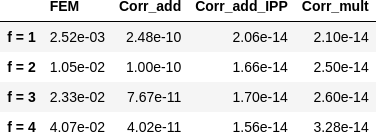
\includegraphics[width=0.8\linewidth]{"corr_ana/tab_errors_fem_circle_nh.png"}
			\captionof{figure}{Relative errors obtained with different methods on the Circle with standard FEM.}
			\label{tab_errors_fem_circle_nh}
		\end{figure} 
	\end{minipage} $\qquad$
	\begin{minipage}{0.48\linewidth} \qquad 
		\begin{figure}[H]
			\centering
			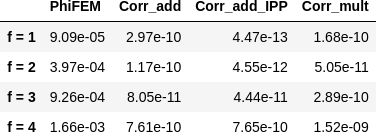
\includegraphics[width=0.8\linewidth]{"corr_ana/tab_errors_phifem_circle_nh.png"}
			\captionof{figure}{Relative errors obtained with different methods on the Circle with $\phi$-FEM.}
			\label{tab_errors_phifem_circle_nh}
		\end{figure} 
	\end{minipage}
	
	\item \textbf{Results on the Square :}
	
	We consider here the Square problem with the solution defined in Section \ref{Corr.pb.square.1}.
	
	\textbf{Homogeneous case :}
	
	We consider here the homogeneous problem (i.e. with $\varphi=0$) and seek to test the various correction methods with standard FEM and $\phi$-FEM methods.
	
	\begin{minipage}{0.48\linewidth}
		\begin{figure}[H]
			\centering
			\includegraphics[width=0.8\linewidth]{"corr_ana/tab_errors_fem_square.png"}
			\captionof{figure}{Relative errors obtained with different methods on the Square with standard FEM.}
			\label{tab_errors_fem_square}
		\end{figure} 
	\end{minipage} $\qquad$
	\begin{minipage}{0.48\linewidth} \qquad 
		\begin{figure}[H]
			\centering
			\includegraphics[width=0.8\linewidth]{"corr_ana/tab_errors_phifem_square.png"}
			\captionof{figure}{Relative errors obtained with different methods on the Square with $\phi$-FEM.}
			\label{tab_errors_phifem_square}
		\end{figure} 
	\end{minipage}
	
	\newpage 
	
	\textbf{Non-homogeneous case :}
	
	We consider here the non-homogeneous problem (i.e. with $\varphi=1$) and seek to test the various correction methods with standard FEM and $\phi$-FEM methods.
	
	\begin{minipage}{0.48\linewidth}
		\begin{figure}[H]
			\centering
			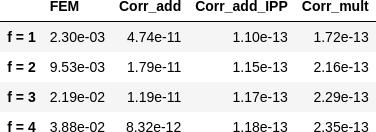
\includegraphics[width=0.8\linewidth]{"corr_ana/tab_errors_fem_square_nh.png"}
			\captionof{figure}{Relative errors obtained with different methods on the Square with standard FEM.}
			\label{tab_errors_fem_square_nh}
		\end{figure} 
	\end{minipage} $\qquad$
	\begin{minipage}{0.48\linewidth} \qquad 
		\begin{figure}[H]
			\centering
			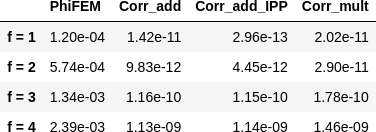
\includegraphics[width=0.8\linewidth]{"corr_ana/tab_errors_phifem_square_nh.png"}
			\captionof{figure}{Relative errors obtained with different methods on the Square with $\phi$-FEM.}
			\label{tab_errors_phifem_square_nh}
		\end{figure} 
	\end{minipage}
\end{enumerate}

It would therefore seem that the various correction methods work in the different cases considered.

\subsubsection{Correction on disturbed solution} \label{Corr.results.disturbed}

Now, let's consider a deliberately disturbed solution. The purpose of this step is to check that the correction solvers also work with a solution that is very close to the real solution, but not exact. In this section, we will consider a manually disturbed solution, i.e. the exact solution to which we've added a small, analytically known perturbation.

As explained above, we begin by considering $\tilde{\phi}$ as a manually perturbed solution defined by
\begin{equation*}
	\tilde{\phi}(x,y)=u_{ex}(x,y)+\epsilon P(x,y)
\end{equation*}
where $u_{ex}$ defines the exact solution to the problem, $P$ the perturbation applied to it and $\epsilon$ is a real number that allows the amplitude of the perturbation to be easily increased or decreased. 

\begin{Rem}
	Notice that by taking $\epsilon=0$, we return to the case of correction on an exact solution presented in Section \ref{Corr.results.ana}. 
\end{Rem}

In our case, we will choose to consider $P$ as being of the same form as our exact solution (defined with different parameters), but we could very well consider a completely different perturbation. 

\begin{Rem}
	Note that the form of the perturbation has a huge influence on the accuracy of the solvers, and that the difficulty lies in the following cases where its expression is not explicitly known (as in the case of $\phi$-FEM in Section \ref{Corr.results.phifem} or FNO in Section \ref{Corr.results.FNO}).
\end{Rem}

In the case of Circle geometry where we consider the problem \ref{Corr.pb.circle.1}, the perturbation will be defined by
\begin{equation*}
	P(x,y)=S_p\times\sin\left(8\pi f_p\left((x-0.5)^2+(y-0.5)^2\right)+\varphi_p\right)
\end{equation*}
where $S_p\in[0,1]$ is the amplitude of the signal, $f_p\in\mathbb{N}$ can be associated with the "frequency" of the signal and $\varphi_p\in[0,1]$ the phase at the origin.

In the case of Square geometry where we consider the problem \ref{Corr.pb.square.1}, the perturbation will be defined by
\begin{equation*}
	P(x,y)=S_p\times\sin\left(2\pi f_px+\varphi_p\right)\times\sin\left(2\pi f_py+\varphi_p\right)
\end{equation*}
where $S_p\in[0,1]$ is the amplitude of the signal, $f_p\in\mathbb{N}$ can be associated with the "frequency" of the signal and $\varphi_p\in[0,1]$ the phase at the origin.

\begin{Rem}
	Note that for the boundary conditions of the solution to be satisfied, i.e. for $\tilde{\phi}=u_{ex}$ on $\Gamma$, it is essential that $P=0$ on $\Gamma$. In the case of both circle and square, we will then take $\varphi_p=0$.
\end{Rem}

Recall the relative errors obtained by standard FEM and $\phi$-FEM on the circle and on the square for frequencies $f\in\{1,2,3,4\}$ for the homogeneous  (Figure \ref{norms}) and non-homogeneous problem  (Figure \ref{norms_nh}).

\begin{minipage}{0.48\linewidth}
	\begin{figure}[H]
		\centering
		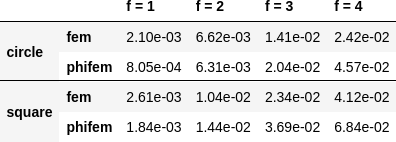
\includegraphics[width=0.8\linewidth]{"corr_pert/diff_eps/norms.png"}
		\captionof{figure}{Table summarizing the errors obtained by standard FEM and $\phi$-FEM on the circle and the square (homogeneous case).}
		\label{norms}
	\end{figure} 
\end{minipage} $\qquad$
\begin{minipage}{0.48\linewidth}
	\begin{figure}[H]
		\centering
		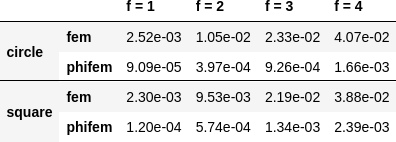
\includegraphics[width=0.8\linewidth]{"corr_pert/diff_eps/norms_nh.png"}
		\captionof{figure}{Table summarizing the errors obtained by standard FEM and $\phi$-FEM on the circle and the square (non-homogeneous case).}
		\label{norms_nh}
	\end{figure} 
\end{minipage}

\begin{Rem}
	In the previous results, we use the direct method to impose the edge conditions with $\phi$-FEM.
\end{Rem}

\paragraph{Results with differents $\epsilon$} \label{Corr.results.disturbed.eps} 

The aim of this section is to test correction by addition (without IPP) and correction by multiplication by varying the amplitude of the perturbation (in other words, by varying $\epsilon$). 

We will try to separate the cases according to the frequencies considered. In other words, for $f,f_p\in\{1,2,3,4\}$, we're interested in the following three cases. The first is the case where the solution frequency is greater than the perturbation frequency ($f>f_p$), i.e. a highly variable solution and a less variable perturbation. The second is where the solution and perturbation frequencies are equal ($f=f_p$), i.e. the solution and perturbation have the same variability. The last category covers cases where the perturbation is "nastier" than the solution, i.e. it has a higher frequency than the solution ($f<f_p$). 

In this section, we will consider for the circle the solution defined in Section \ref{Corr.pb.circle.1} and for the square the solution defined in Section \ref{Corr.pb.square.1}.

\textbf{Results with standard FEM :}

First we will consider the standard FEM method on the homogeneous case (i.e. with $\varphi=0$) and then on the non-homogeneous case (i.e. with $\varphi=1$).

\begin{enumerate}[label=\textbullet]
	\item \textbf{Results on the homogeneous case :}
	
	First, we consider the correction by adding (without IPP) on the Circle problem (Figure \ref{corr_pert_fem_circle_add}) and on the Square problem (Figure \ref{corr_pert_fem_square_add}).
	
	\begin{minipage}{0.48\linewidth}
		\begin{figure}[H]
			\centering
			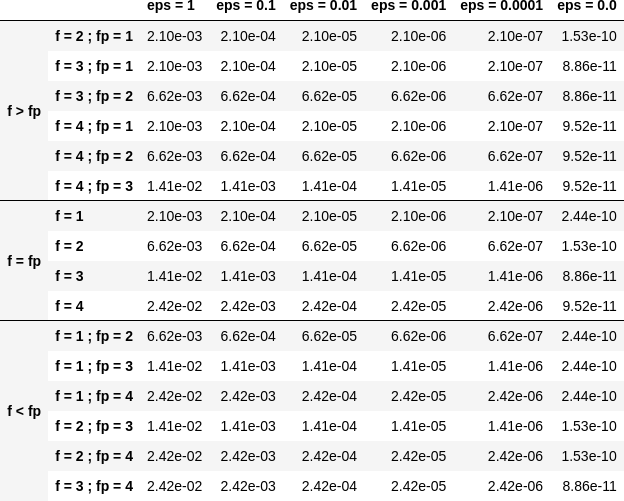
\includegraphics[width=0.95\linewidth]{"corr_pert/diff_eps/fem_circle_add.png"}
			\captionof{figure}{Correction by adding on the Circle with standard FEM in the homogeneous case.}
			\label{corr_pert_fem_circle_add}
		\end{figure} 
	\end{minipage} $\qquad$
	\begin{minipage}{0.48\linewidth}
		\begin{figure}[H]
			\centering
			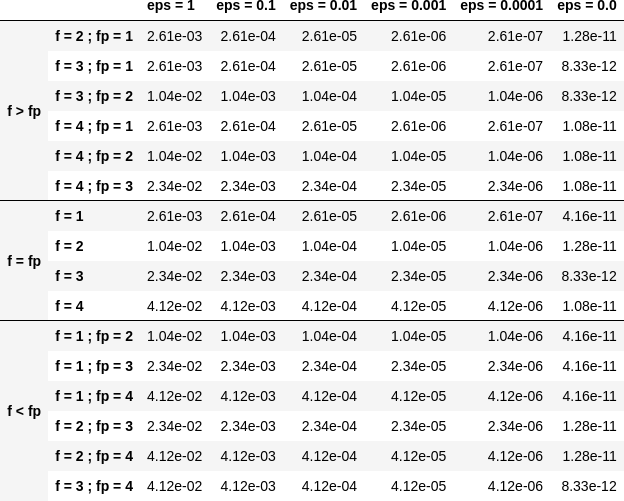
\includegraphics[width=0.95\linewidth]{"corr_pert/diff_eps/fem_square_add.png"}
			\captionof{figure}{Correction by adding on the Square with standard FEM in the homogeneous case.}
			\label{corr_pert_fem_square_add}
		\end{figure} 
	\end{minipage}
	
	Then, we consider the correction by multiplying on the Circle problem (Figure \ref{corr_pert_fem_circle_mult}) and on the Square problem (Figure \ref{corr_pert_fem_square_mult}).
	
	\begin{minipage}{0.48\linewidth}
		\begin{figure}[H]
			\centering
			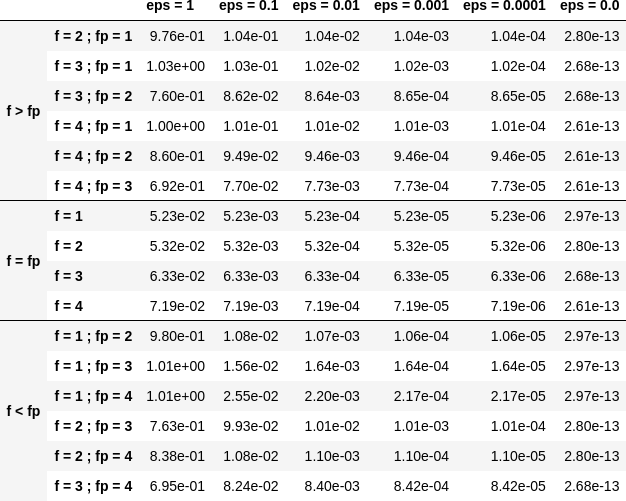
\includegraphics[width=0.95\linewidth]{"corr_pert/diff_eps/fem_circle_mult.png"}
			\captionof{figure}{Correction by multiplying on the Circle with standard FEM in the homogeneous case.}
			\label{corr_pert_fem_circle_mult}
		\end{figure} 
	\end{minipage} $\qquad$
	\begin{minipage}{0.48\linewidth}
		\begin{figure}[H]
			\centering
			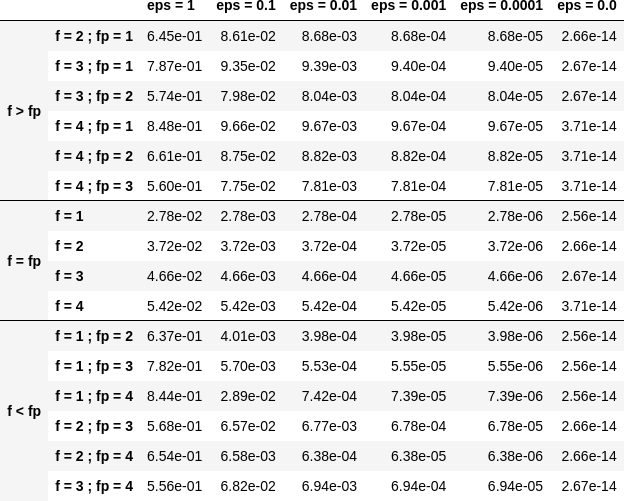
\includegraphics[width=0.95\linewidth]{"corr_pert/diff_eps/fem_square_mult.png"}
			\captionof{figure}{Correction by multiplying on the Square with standard FEM in the homogeneous case.}
			\label{corr_pert_fem_square_mult}
		\end{figure} 
	\end{minipage}
	
	\textbf{\textit{Observation :}} We can make a few comments on the results obtained:
	\begin{itemize}
		\item  First of all, it would therefore seem that, overall, the smaller the perturbation applied (i.e. the smaller the $\epsilon$), the more efficient the addition and multiplication correction solvers are in terms of accuracy.
		\item Then, it would appear that, as with the standard FEM and $\phi$-FEM solvers without correction, the more the solution varies (i.e. the larger $f$), the greater the error. This is a fairly intuitive result, since the more the solution varies, the more points are needed to approximate it.
		\item It would also seem that for $\epsilon=1$ (i.e. a large perturbation), the $\epsilon$ parameter has a greater impact on the multiplicative corrector than on the additive corrector. We explained earlier the benefits of elevating the problem, which could be beneficial here. Results on elevation will be presented in the Section \ref{Corr.results.disturbed.reh}.
		\item In view of the results obtained here, it would also appear that, overall, correction by addition is more effective than correction by multiplication. Moreover, correction by addition has more advantages than correction by multiplication. In particular, if the solution cancels out on the domain, correction by multiplication will require elevating the problem sufficiently so that it no longer cancels out, unlike correction by addition.
		\item There is one final and rather important point to make. In fact, if we take a closer look at the results, we can see that in the case of correction by adding, the errors only seem to depend on the frequency of the perturbation and not on that of the solution (at a fixed $\epsilon$). This is a result that has been explained theoretically in the case of correction by multiplication on a elevated problem in the Section \ref{Corr.theo_results.reh} (for $m$ large, similar to correction by addition as explained above). Thus, as we have shown (in Section \ref{Corr.theo_results.comp_add_reh}) that for $m$ large, the error of correction by multiplication on a elevated problem converges to the error of correction by addition, we recover this result on correction by addition.
	\end{itemize}
	
	\item \textbf{Results on the non-homogeneous case :}
	
	First, we consider the correction by adding (without IPP) on the Circle problem (Figure \ref{corr_pert_fem_circle_add_nh}) and on the Square problem (Figure \ref{corr_pert_fem_square_add_nh}).
	
	\begin{minipage}{0.48\linewidth}
		\begin{figure}[H]
			\centering
			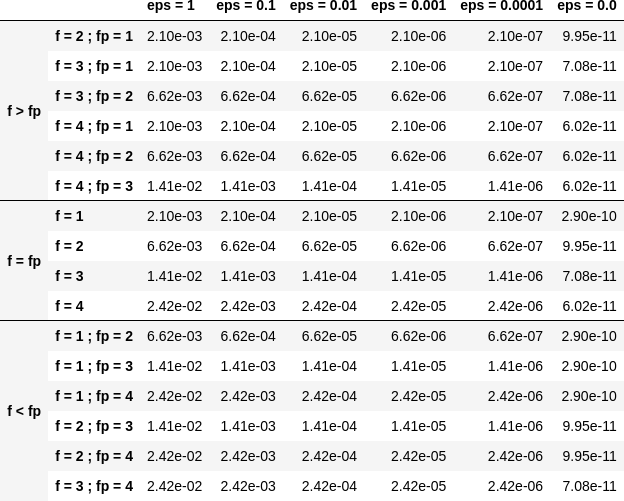
\includegraphics[width=0.9\linewidth]{"corr_pert/diff_eps/fem_circle_add_nh.png"}
			\captionof{figure}{Correction by adding on the Circle with standard FEM in the non-homogeneous case.}
			\label{corr_pert_fem_circle_add_nh}
		\end{figure} 
	\end{minipage} $\qquad$
	\begin{minipage}{0.48\linewidth}
		\begin{figure}[H]
			\centering
			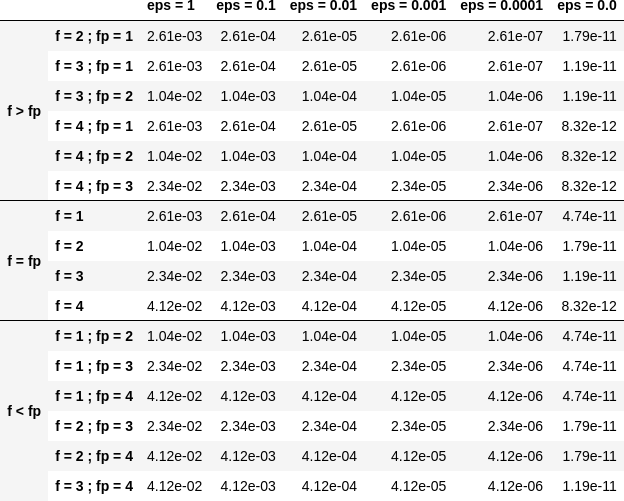
\includegraphics[width=0.9\linewidth]{"corr_pert/diff_eps/fem_square_add_nh.png"}
			\captionof{figure}{Correction by adding on the Square with standard FEM in the non-homogeneous case.}
			\label{corr_pert_fem_square_add_nh}
		\end{figure} 
	\end{minipage}
	
	Then, we consider the correction by multiplying on the Circle problem (Figure \ref{corr_pert_fem_circle_mult_nh}) and on the Square problem (Figure \ref{corr_pert_fem_square_mult_nh}).
	
	\begin{minipage}{0.48\linewidth}
		\begin{figure}[H]
			\centering
			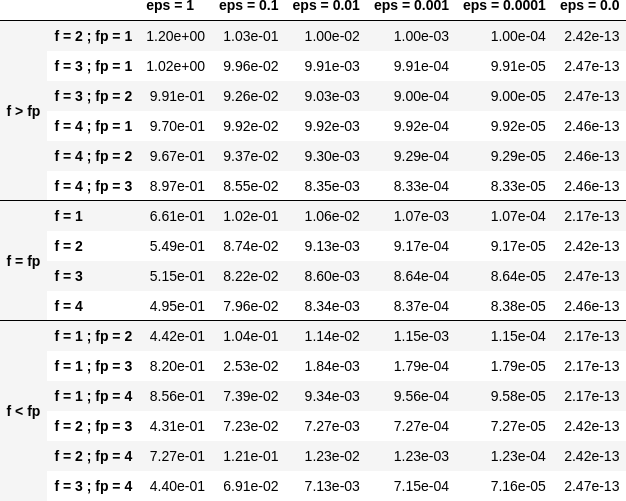
\includegraphics[width=0.95\linewidth]{"corr_pert/diff_eps/fem_circle_mult_nh.png"}
			\captionof{figure}{Correction by multiplying on the Circle with standard FEM in the non-homogeneous case.}
			\label{corr_pert_fem_circle_mult_nh}
		\end{figure} 
	\end{minipage} $\qquad$
	\begin{minipage}{0.48\linewidth}
		\begin{figure}[H]
			\centering
			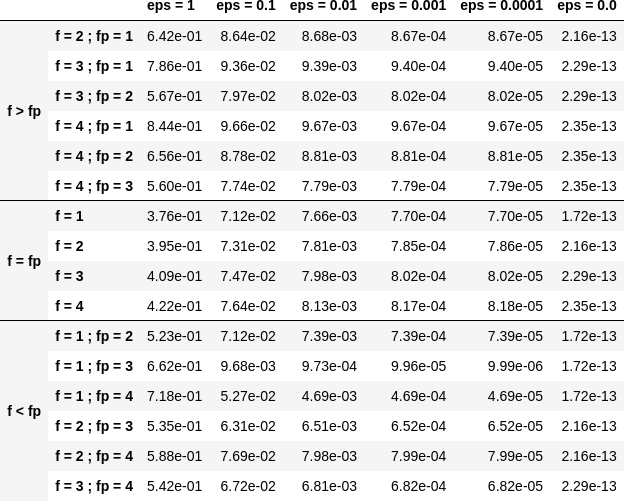
\includegraphics[width=0.95\linewidth]{"corr_pert/diff_eps/fem_square_mult_nh.png"}
			\captionof{figure}{Correction by multiplying on the Square with standard FEM in the non-homogeneous case.}
			\label{corr_pert_fem_square_mult_nh}
		\end{figure} 
	\end{minipage}
	
	\textbf{\textit{Observation :}} In view of the results obtained, it would appear that the conclusions are the same as for the homogeneous case.
\end{enumerate}

\textbf{Results with $\phi$-FEM :}

Then we will consider the $\phi$-FEM method on the homogeneous case (i.e. with $\varphi=0$) and then on the non-homogeneous case (i.e. with $\varphi=1$).

\begin{enumerate}[label=\textbullet]
	\item \textbf{Results on the homogeneous case :}
	
	First, we consider the correction by adding (without IPP) on the Circle problem (Figure \ref{corr_pert_phifem_circle_add}) and on the Square problem (Figure \ref{corr_pert_phifem_square_add}).
	
	\begin{minipage}{0.48\linewidth}
		\begin{figure}[H]
			\centering
			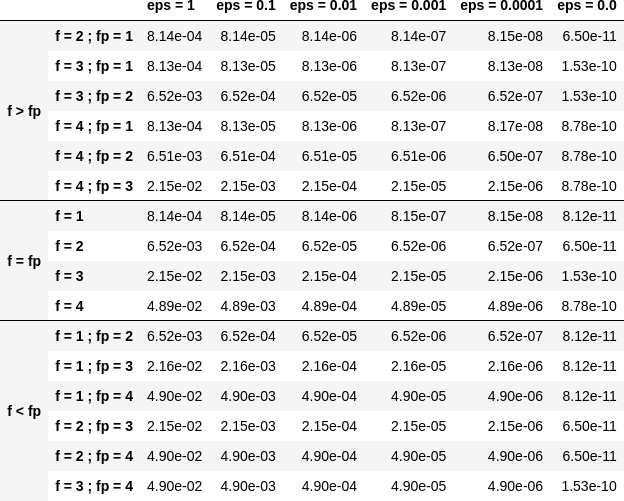
\includegraphics[width=0.95\linewidth]{"corr_pert/diff_eps/phifem_circle_add.png"}
			\captionof{figure}{Correction by adding on the Circle with $\phi$-FEM in the homogeneous case.}
			\label{corr_pert_phifem_circle_add}
		\end{figure} 
	\end{minipage} $\qquad$
	\begin{minipage}{0.48\linewidth}
		\begin{figure}[H]
			\centering
			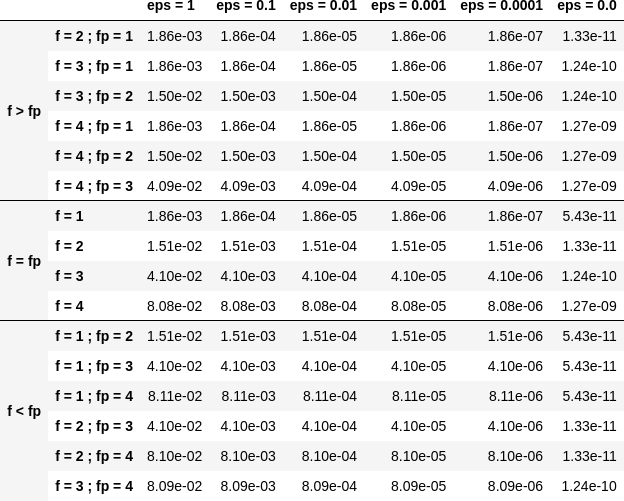
\includegraphics[width=0.95\linewidth]{"corr_pert/diff_eps/phifem_square_add.png"}
			\captionof{figure}{Correction by adding on the Square with $\phi$-FEM in the homogeneous case.}
			\label{corr_pert_phifem_square_add}
		\end{figure} 
	\end{minipage}
	
	Then, we consider the correction by multiplying on the Circle problem (Figure \ref{corr_pert_phifem_circle_mult}) and on the Square problem (Figure \ref{corr_pert_phifem_square_mult}).
	
	\begin{minipage}{0.48\linewidth}
		\begin{figure}[H]
			\centering
			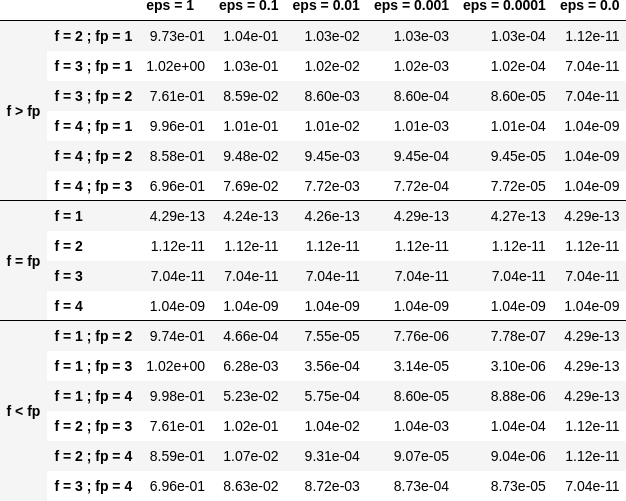
\includegraphics[width=0.9\linewidth]{"corr_pert/diff_eps/phifem_circle_mult.png"}
			\captionof{figure}{Correction by multiplying on the Circle with $\phi$-FEM in the homogeneous case.}
			\label{corr_pert_phifem_circle_mult}
		\end{figure} 
	\end{minipage} $\qquad$
	\begin{minipage}{0.48\linewidth}
		\begin{figure}[H]
			\centering
			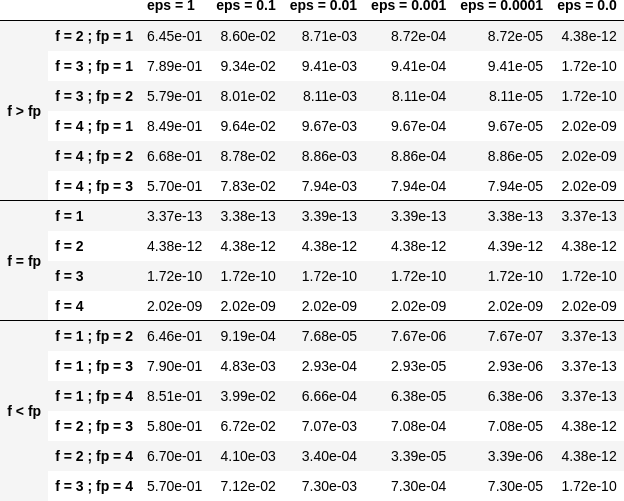
\includegraphics[width=0.9\linewidth]{"corr_pert/diff_eps/phifem_square_mult.png"}
			\captionof{figure}{Correction by multiplying on the Square with $\phi$-FEM in the homogeneous case.}
			\label{corr_pert_phifem_square_mult}
		\end{figure} 
	\end{minipage}
	
	\textbf{\textit{Observation :}} An interesting result can also be observed. Indeed, it seems that in the case where $f=f_p$, the multiplication correction with $\phi$-FEM seems to approach the solution almost perfectly for all $\epsilon$ considered.
	In fact, in the homogeneous case, for $f=f_p$ the perturbation is identical to the solution (i.e. $P=u_{ex}$) and so the solution injected into the correction solvers is of the form
	\begin{equation*}
		\tilde{\phi}=u_{ex}+\epsilon P=(1+\epsilon)u_{ex}
	\end{equation*}
	In the case of correction by multiplication, we have $\tilde{u}=\tilde{\phi}C$. So for $\tilde{u}=u_{ex}$, we must have
	\begin{equation*}
		\tilde{\phi}C=u_{ex} \quad \iff \quad (1+\epsilon)u_{ex}C=u_{ex}
	\end{equation*}
	So if the solution does not cancel out on $\Omega$, we must have
	\begin{equation*}
		C=\frac{1}{1+\epsilon} \quad \text{on } \Omega
	\end{equation*}
	By imposing $C=\frac{1}{1+\epsilon}$ on $\Gamma$ for FEM instead of $C=1$, we should get closer to the $\phi$-FEM results obtained. We can see in Figure \ref{norms_circle_f_eq_fp} and Figure \ref{norms_square_f_eq_fp} that we obtain the expected results for FEM by changing the boundary condition $C=1$ to $C=\frac{1}{1+\epsilon}$.
	
	\begin{minipage}{0.48\linewidth}
		\begin{figure}[H]
			\centering
			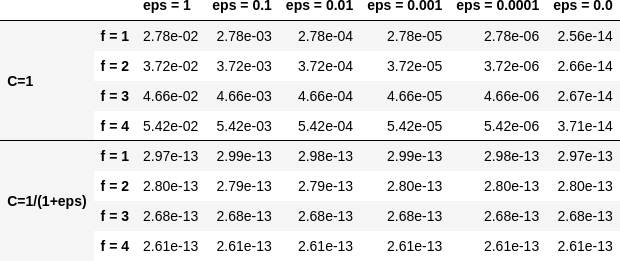
\includegraphics[width=0.8\linewidth]{"corr_pert/diff_eps/norms_circle_f_eq_fp.png"}
			\captionof{figure}{Results by changing FEM boundary conditions on the circle.}
			\label{norms_circle_f_eq_fp}
		\end{figure} 
	\end{minipage} $\qquad$
	\begin{minipage}{0.48\linewidth}
		\begin{figure}[H]
			\centering
			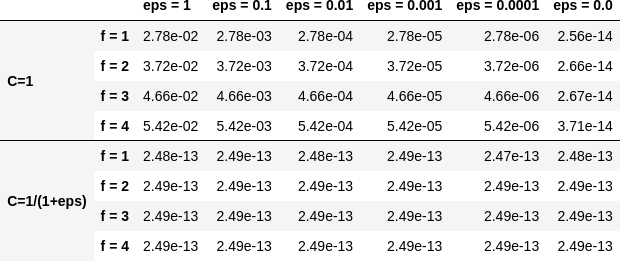
\includegraphics[width=0.8\linewidth]{"corr_pert/diff_eps/norms_square_f_eq_fp.png"}
			\captionof{figure}{Results by changing FEM boundary conditions on the square.}
			\label{norms_square_f_eq_fp}
		\end{figure} 
	\end{minipage}
	
	\begin{Rem}
		It should be noted, however, that in practice, for example in the case where $\tilde{\phi}$ is a $\phi$-FEM solution or an FNO output, this case is not very realistic. There's no reason to expect the form of the perturbation created by the $\phi$-FEM solver or by the FNO to be exactly identical to the solution under consideration.
	\end{Rem}
	
	\item \textbf{Results on the non-homogeneous case :}
	
	First, we consider the correction by adding (without IPP) on the Circle problem (Figure \ref{corr_pert_phifem_circle_add_nh}) and on the Square problem (Figure \ref{corr_pert_phifem_square_add_nh}).
	
	\begin{minipage}{0.48\linewidth}
		\begin{figure}[H]
			\centering
			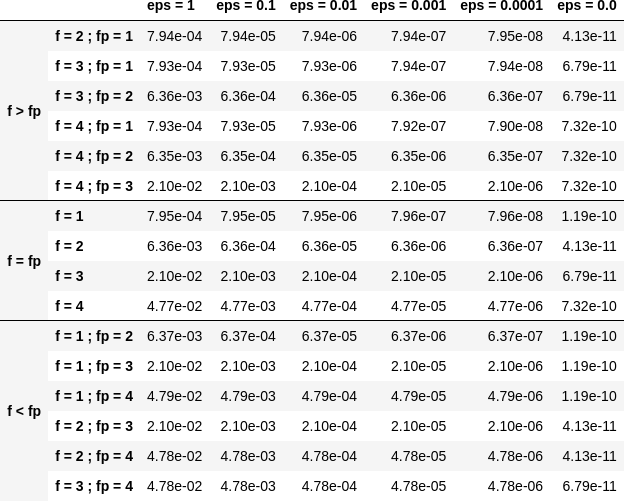
\includegraphics[width=0.9\linewidth]{"corr_pert/diff_eps/phifem_circle_add_nh.png"}
			\captionof{figure}{Correction by adding on the Circle with $\phi$-FEM in the non-homogeneous case.}
			\label{corr_pert_phifem_circle_add_nh}
		\end{figure} 
	\end{minipage} $\qquad$
	\begin{minipage}{0.48\linewidth}
		\begin{figure}[H]
			\centering
			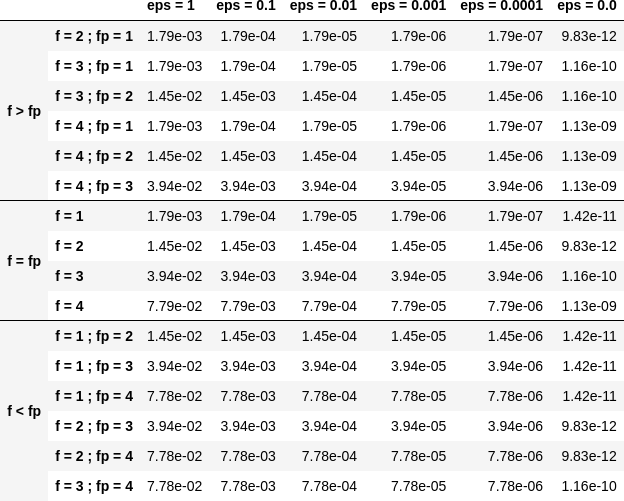
\includegraphics[width=0.9\linewidth]{"corr_pert/diff_eps/phifem_square_add_nh.png"}
			\captionof{figure}{Correction by adding on the Square with $\phi$-FEM in the non-homogeneous case.}
			\label{corr_pert_phifem_square_add_nh}
		\end{figure} 
	\end{minipage}
	
	Then, we consider the correction by multiplying on the Circle problem (Figure \ref{corr_pert_phifem_circle_mult_nh}) and on the Square problem (Figure \ref{corr_pert_phifem_square_mult_nh}). We start by considering the same $\phi$-FEM scheme as in the homogeneous case, i.e. here we don't impose any edge conditions.
	
	\begin{minipage}{0.48\linewidth}
		\begin{figure}[H]
			\centering
			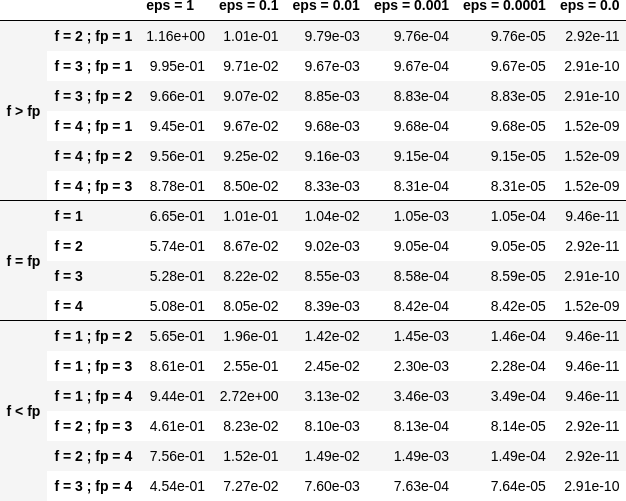
\includegraphics[width=0.8\linewidth]{"corr_pert/diff_eps/phifem_circle_mult_nh.png"}
			\captionof{figure}{Correction by multiplying on the Circle with $\phi$-FEM in the non-homogeneous case.}
			\label{corr_pert_phifem_circle_mult_nh}
		\end{figure} 
	\end{minipage} $\qquad$
	\begin{minipage}{0.48\linewidth}
		\begin{figure}[H]
			\centering
			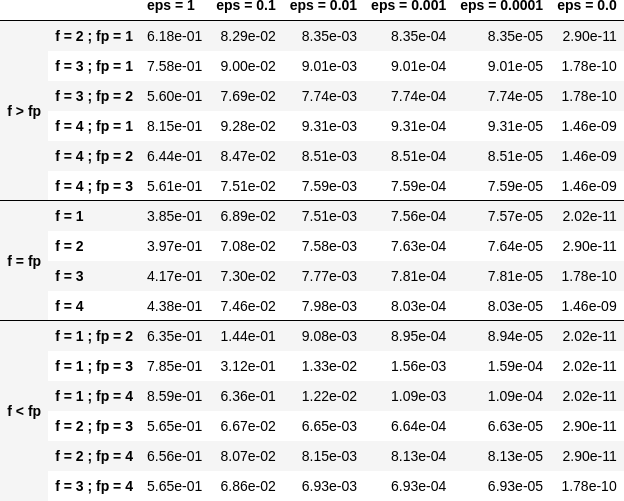
\includegraphics[width=0.8\linewidth]{"corr_pert/diff_eps/phifem_square_mult_nh.png"}
			\captionof{figure}{Correction by multiplying on the Square with $\phi$-FEM in the non-homogeneous case.}
			\label{corr_pert_phifem_square_mult_nh}
		\end{figure} 
	\end{minipage}
	
	\textbf{\textit{Observation :}} We note that the multiplicative corrector using $\phi$-FEM seems to succeed, in a similar way to the homogeneous case, to correct the non-homogeneous problem without imposing the boundary conditions. In fact, there's a subtlety to the scheme we're considering here. Unlike $\phi$-FEM (without correction), the scheme is written on $\tilde{\phi}$, which is non-zero at the boundary, and not on $\phi$, which is zero at the boundary. This could explain this result, whereas in the case of $\phi$-FEM (without correction), we can't avoid imposing boundary conditions.
	
	We will now use the direct method to impose the boundary condition. For this method, we're tempted to consider the solution $\tilde{u}=\tilde{\phi}C+g$ as the solution to the multiplication correction problem. In fact, unlike the classic $\phi$-FEM method, the $\tilde{\phi}$ function that replaces our level-set in the formulation is non-zero at the boundary and so, by imposing $C=1$ at the boundary, we'd have $\tilde{u}=2g$. To avoid this problem, we will raise the problem by $-g$ and consider $\tilde{u}=(\tilde{\phi}-g)C+g$. We will test this method on the circle (Figure \ref{corr_pert_phifem_circle_mult_direct_nh}) and on the square (Figure \ref{corr_pert_phifem_square_mult_direct_nh}).
	
	\begin{minipage}{0.48\linewidth}
		\begin{figure}[H]
			\centering
			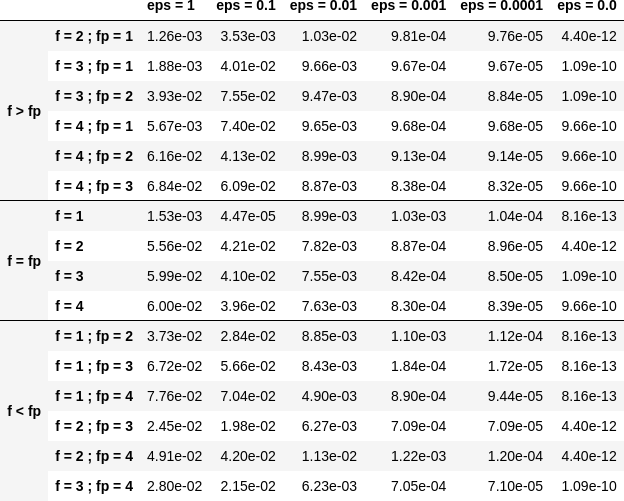
\includegraphics[width=0.8\linewidth]{"corr_pert/diff_eps/phifem_circle_mult_direct_nh.png"}
			\captionof{figure}{Correction by multiplying on the Circle with $\phi$-FEM in the non-homogeneous case (direct method).}
			\label{corr_pert_phifem_circle_mult_direct_nh}
		\end{figure} 
	\end{minipage} $\qquad$
	\begin{minipage}{0.48\linewidth}
		\begin{figure}[H]
			\centering
			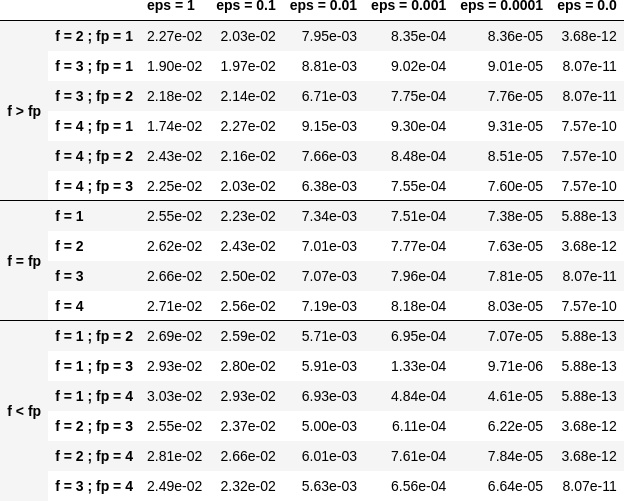
\includegraphics[width=0.8\linewidth]{"corr_pert/diff_eps/phifem_square_mult_direct_nh.png"}
			\captionof{figure}{Correction by multiplying on the Square with $\phi$-FEM in the non-homogeneous case (direct method).}
			\label{corr_pert_phifem_square_mult_direct_nh}
		\end{figure} 
	\end{minipage}
	
	We're now going to test imposing boundary conditions with the dual method on the circle (Figure \ref{corr_pert_phifem_circle_mult_dual_nh}) and on the square (Figure \ref{corr_pert_phifem_square_mult_dual_nh}).
	
	\begin{minipage}{0.48\linewidth}
		\begin{figure}[H]
			\centering
			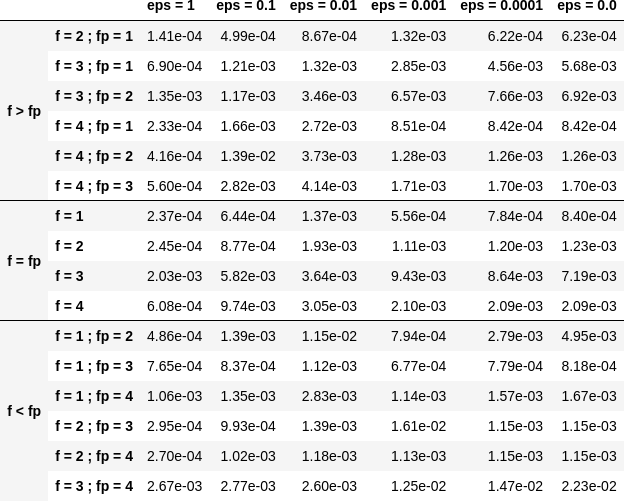
\includegraphics[width=0.8\linewidth]{"corr_pert/diff_eps/phifem_circle_mult_dual_nh.png"}
			\captionof{figure}{Correction by multiplying on the Circle with $\phi$-FEM in the non-homogeneous case (dual method).}
			\label{corr_pert_phifem_circle_mult_dual_nh}
		\end{figure} 
	\end{minipage} $\qquad$
	\begin{minipage}{0.48\linewidth}
		\begin{figure}[H]
			\centering
			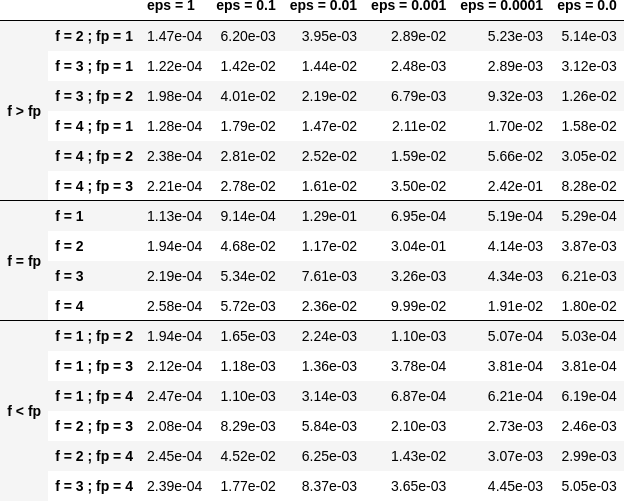
\includegraphics[width=0.8\linewidth]{"corr_pert/diff_eps/phifem_square_mult_dual_nh.png"}
			\captionof{figure}{Correction by multiplying on the Square with $\phi$-FEM in the non-homogeneous case (dual method).}
			\label{corr_pert_phifem_square_mult_dual_nh}
		\end{figure} 
	\end{minipage}
	
	\textbf{\textit{Observation :}} It seems that by imposing the boundary conditions with the direct method, the errors are better when $\epsilon$ is a bit large, especially for $\epsilon=1$. For the dual method, it seems also works for imposing boundary conditions. However, we can see that it can become slightly stagnant when $\epsilon$ is decreased. It's possible that changing the stabilization parameters could have an impact here.
	
\end{enumerate}

\paragraph{Results on the elevated problem} \label{Corr.results.disturbed.reh} 

In this section, we aim to show numerically the interest of elevating the problem. To do this, we will consider the case of the circle with the solution defined in Section \ref{Corr.pb.circle.1} and the case of the square with the solution defined in Section \ref{Corr.pb.square.1}. We will choose the homogeneous case (i.e. with $\varphi=0$) with $S=0.5$ and set $\epsilon=10^{-3}$.

\textbf{Results with FEM :}

Here, we consider some of the cases considered above, in order to test the correction by multiplying on an elevating problem with FEM (theoretical result presented in Section \ref{Corr.method.mult_reh}). We will test this method on the circle (Figure \ref{corr_pert_fem_circle_reh} and Figure \ref{corr_pert_fem_circle_reh_fig}) and on the square (Figure \ref{corr_pert_fem_square_reh} and Figure \ref{corr_pert_fem_square_reh_fig}) for selected frequencies and by varying $m$.

\begin{minipage}{0.48\linewidth}
	\begin{figure}[H]
		\centering
		\includegraphics[width=\linewidth]{"corr_pert/rehaussement/tab_errors_fem_circle.png"}
		\captionof{figure}{Correction by multiplying on the elevated problem on the Circle with FEM.}
		\label{corr_pert_fem_circle_reh}
	\end{figure} 
\end{minipage} $\qquad$
\begin{minipage}{0.48\linewidth}
	\begin{figure}[H]
		\centering
		\includegraphics[width=\linewidth]{"corr_pert/rehaussement/tab_errors_fem_square.png"}
		\captionof{figure}{Correction by multiplying on the elevated problem on the Square with FEM.}
		\label{corr_pert_fem_square_reh}
	\end{figure} 
\end{minipage}

\begin{minipage}{0.48\linewidth}
	\begin{figure}[H]
		\centering
		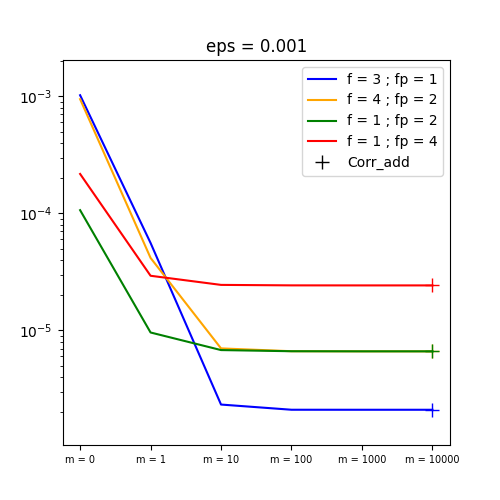
\includegraphics[width=0.8\linewidth]{"corr_pert/rehaussement/fig_fem_circle.png"}
		\captionof{figure}{Representation of the results on the Circle with FEM.}
		\label{corr_pert_fem_circle_reh_fig}
	\end{figure} 
\end{minipage} $\qquad$
\begin{minipage}{0.48\linewidth}
	\begin{figure}[H]
		\centering
		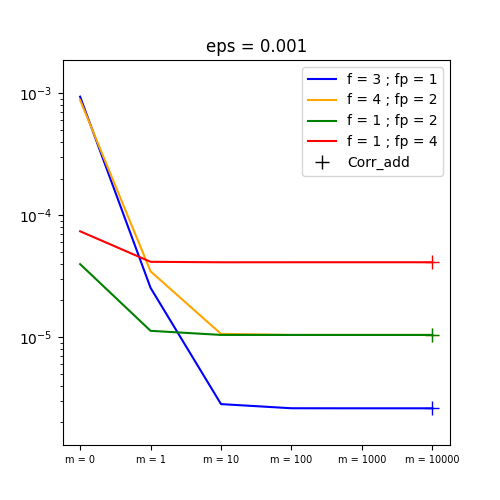
\includegraphics[width=0.8\linewidth]{"corr_pert/rehaussement/fig_fem_square.png"}
		\captionof{figure}{Representation of the results on the Square with FEM.}
		\label{corr_pert_fem_square_reh_fig}
	\end{figure} 
\end{minipage}

\textbf{Observation :} The numerical results obtained on the circle in Figure \ref{corr_pert_fem_circle_reh} and on the square \ref{corr_pert_fem_square_reh}, seem to show that the higher we raise the problem, the better the error. Furthermore, as explained in Section \ref{Corr.theo_results.comp_add_reh}, we can see that by increasing $m$, the error converges to the error obtained with the correction by adding (because the solution itself converges to the solution obtained with the correction by adding). 

\textbf{Results with $\phi$-FEM :}

Now we to test the correction by multiplying on an elevating problem with $\phi$-FEM. We will test this method on the circle (Figure \ref{corr_pert_phifem_circle_reh} and Figure \ref{corr_pert_phifem_circle_reh_fig}) and on the square (Figure \ref{corr_pert_phifem_square_reh} and Figure \ref{corr_pert_phifem_square_reh_fig}) for selected frequencies and by varying $m$. Here, we're using the same scheme as in the homogeneous case, i.e. we're not going to impose the boundary conditions using the direct or dual method. 

\begin{minipage}{0.48\linewidth}
	\begin{figure}[H]
		\centering
		\includegraphics[width=\linewidth]{"corr_pert/rehaussement/tab_errors_phifem_circle.png"}
		\captionof{figure}{Correction by multiplying on the elevated problem on the Circle with $\phi$-FEM.}
		\label{corr_pert_phifem_circle_reh}
	\end{figure} 
\end{minipage} $\qquad$
\begin{minipage}{0.48\linewidth}
	\begin{figure}[H]
		\centering
		\includegraphics[width=\linewidth]{"corr_pert/rehaussement/tab_errors_phifem_square.png"}
		\captionof{figure}{Correction by multiplying on the elevated problem on the Square with $\phi$-FEM.}
		\label{corr_pert_phifem_square_reh}
	\end{figure} 
\end{minipage}

\begin{minipage}{0.48\linewidth}
	\begin{figure}[H]
		\centering
		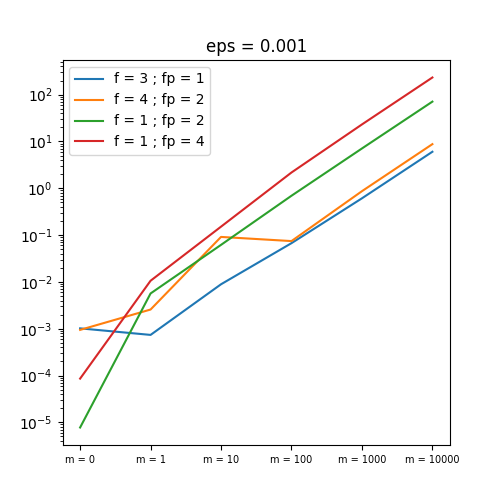
\includegraphics[width=0.8\linewidth]{"corr_pert/rehaussement/fig_phifem_circle.png"}
		\captionof{figure}{Representation of the results on the Circle with FEM.}
		\label{corr_pert_phifem_circle_reh_fig}
	\end{figure} 
\end{minipage} $\qquad$
\begin{minipage}{0.48\linewidth}
	\begin{figure}[H]
		\centering
		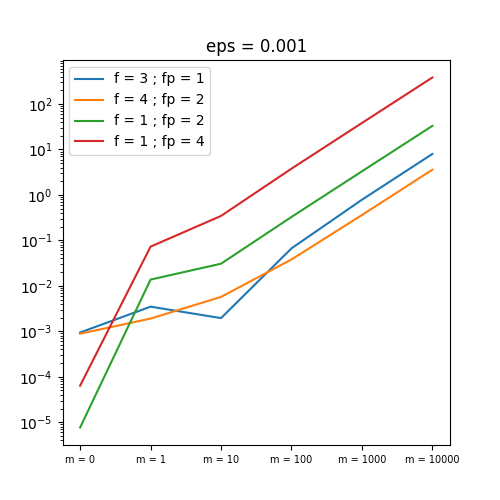
\includegraphics[width=0.8\linewidth]{"corr_pert/rehaussement/fig_phifem_square.png"}
		\captionof{figure}{Representation of the results on the Square with FEM.}
		\label{corr_pert_phifem_square_reh_fig}
	\end{figure} 
\end{minipage}

Now, we impose the boundary conditions using the dual method, always considering the circle (Figure \ref{corr_pert_phifem_circle_dual_reh} and Figure \ref{corr_pert_phifem_circle_dual_reh_fig}) and on the square (Figure \ref{corr_pert_phifem_square_dual_reh} and Figure \ref{corr_pert_phifem_square_dual_reh_fig}) for selected frequencies and by varying $m$.

\begin{minipage}{0.48\linewidth}
	\begin{figure}[H]
		\centering
		\includegraphics[width=\linewidth]{"corr_pert/rehaussement/tab_errors_phifem_circle_dual.png"}
		\captionof{figure}{Correction by multiplying on the elevated problem on the Circle with FEM.}
		\label{corr_pert_phifem_circle_dual_reh}
	\end{figure} 
\end{minipage} $\qquad$
\begin{minipage}{0.48\linewidth}
	\begin{figure}[H]
		\centering
		\includegraphics[width=\linewidth]{"corr_pert/rehaussement/tab_errors_phifem_square_dual.png"}
		\captionof{figure}{Correction by multiplying on the elevated problem on the Square with FEM.}
		\label{corr_pert_phifem_square_dual_reh}
	\end{figure} 
\end{minipage}

\begin{minipage}{0.48\linewidth}
	\begin{figure}[H]
		\centering
		\includegraphics[width=\linewidth]{"corr_pert/rehaussement/fig_phifem_circle_dual.png"}
		\captionof{figure}{Representation of the results on the Circle with FEM.}
		\label{corr_pert_phifem_circle_dual_reh_fig}
	\end{figure} 
\end{minipage} $\qquad$
\begin{minipage}{0.48\linewidth}
	\begin{figure}[H]
		\centering
		\includegraphics[width=\linewidth]{"corr_pert/rehaussement/fig_phifem_square_dual.png"}
		\captionof{figure}{Representation of the results on the Square with FEM.}
		\label{corr_pert_phifem_square_dual_reh_fig}
	\end{figure} 
\end{minipage}

\textbf{\textit{Observation :}} It would appear that, in the case of multiplication correction on an elevated problem, we are forced to impose the boundary conditions using one of the two methods, unlike multiplication correction without elevation. By imposing boundary conditions using the dual method, it seems that in the case where the frequency of the solution is greater than the frequency of the perturbation (for $f>f_p$), we do reduce the error by increasing $m$, but it doesn't seem as efficient as in the case with FEM. Indeed, in all the cases considered here, correction by addition gives much better results. Moreover, for $f< f_p$, it would appear that the enhancement is the opposite of the expected effect.

\begin{Rem}
	Note that the direct method is not applicable in the case of this problem because, as explained in the case of correction without elevation on a non-homogeneous problem, we are in some ways returning to the homogeneous problem. In fact, if we consider 
	\begin{equation*}
		\hat{u}=(\hat{\phi}-g-m)C+(g+m)=(\tilde{\phi}-g)C+(g+m)
	\end{equation*}
	with $g=0$ because we've placed ourselves in the homogeneous case, which amounts to solving the problem without elevation.
\end{Rem}

\subsubsection{Correction on $\phi$-FEM solution} \label{Corr.results.phifem}

\modif{Then we will look at correcting a disturbed solution for which we don't know the form of the perturbation. A $\phi$-FEM solution can be considered for injection into correction solvers.}

\subsubsection{Correction with FNO} \label{Corr.results.FNO}

In this section, we will consider the problem presented in Section \ref{Corr.pb.circle.2}, where we take as geometry the circle and $f$ Gaussian. In practice, this is a very probable case, i.e. one in which no exact solution is known. As explained above, we will take an over-refined solution (calculated with FEM) as our reference solution. 

We want to train an FNO to predict the solutions of the problem under consideration and test the correction on its predictions. To do this, we will follow the steps presented in Section \ref{FNO.application}. In the following, we will choose an FNO with 4 Fourier layers.

\paragraph{Training the FNO} \label{Corr.results.FNO.Training}

We start by training the FNO with $\phi$-FEM solutions. To do this, we consider a number of training data $n_{data}$ and perform the following steps:
\begin{enumerate}[label=\textbullet]
	\item First, we randomly generate a sample of parameters defined by
	\begin{equation*}
		\{\mu_0^{(i)},\mu_1^{(i)},\sigma^{(i)}\}_{i=1,\dots,n_{data}}
	\end{equation*}
	with $\sigma \sim \mathcal{U}([0.1,0.6])$ and $\mu_0, \mu_1 \sim \mathcal{U}([0.5-\sqrt{2}/4, 0.5+\sqrt{2}/4])$ with the condition $\phi(\mu_0, \mu_1) < -0.05$.
	
	\begin{Rem}
		The condition $\phi(\mu_0, \mu_1) < -0.05$ ensures that the center $(\mu_0, \mu_1)$ of the Gaussian is inside the domain.
	\end{Rem}
	
	From the parameter sample created, we can generate a Gaussian sample defined by
	\begin{equation*}
		\{f_i\}_{i=1,\dots,n_{data}}=\left\{\exp\left(-\frac{(x-\mu_0^{(i)})^2 + (y-\mu_1^{(i)})^2}{2(\sigma^{(i)})^2}\right)\right\}_{i=1,\dots,n_{data}}
	\end{equation*}
	
	\begin{Rem}
		As explained in Section \ref{FNO.application}, each Gaussian is in fact evaluated at the nodes of our grid, so they are 2D matrices of size $n_{vert}\times n_{vert}$.
		
		We can also consider the degrees of freedom $\mathbb{P}_2$, which also form a regular grid, as they are composed of the nodes as well as the midpoints of each segment. So our matrices will be of size $n_{dofs}\times n_{dofs}$ (with $n_{dofs}=2n_{vert}-1$). In the following, we will choose $n_{vert}$=32 and thus $n_{dofs}=63$.
	\end{Rem}
	
	In our case, the geometry is fixed (the circle with center $(0.5,0.5)$ and radius $\sqrt{2}/4$), so we will not have a level-set collection in our training data. Similarly, we choose to consider the homogeneous problem and so, since $g=0$ on $\Gamma$, we won't have a collection of Dirichlet conditions in our training data either.
	
	\item We can now use the $\phi$-FEM scheme associated with the Poisson problem with homogeneous Dirichlet condition defined in Section \ref{FEMs.PhiFEM.Pres.method} to solve for each $i=1,\dots,n_{data}$, the problem
	\begin{equation*}
		\left\{
		\begin{aligned}
			-\Delta (\phi w_i) &= f_i, \; &&\text{in } \; \Omega, \\
			u_i&=0, \; &&\text{on } \; \partial\Omega,
		\end{aligned}
		\right.
	\end{equation*}
	with $u_i=\phi w_i$.
	
	We thus have a collection of $\phi$-FEM solutions of the problem defined by
	\begin{equation*}
		\{u_i\}_{i=1,\dots,n_{data}}=\{\phi w_i\}_{i=1,\dots,n_{data}}
	\end{equation*}
	
	\item From the previous collections, we can now create the X\_train and Y\_train samples that will enable us to train the FNO. we will start by performing a kind of pre-processing on our data (explained in Section \ref{FNO.application}) by normalizing the source term collection. We thus consider
	\begin{equation*}
		f_{i,norm} = \frac{f_i}{max_{j=1},\dots,n_{data} ||f_j||_{L^2(\mathcal{O})}}, \quad \forall i\in 1,\dots,n_{data}.
	\end{equation*}
	We can now define X\_train as follows
	\begin{equation*}
		X\_train =  \left\{f_{i,norm},F_{i,norm}^{(x)},F_{i,norm}^{(y)},F_{i,norm}^{(xx)},F_{i,norm}^{(yy)}\right\}_{i=1,\dots,n_{data}}
	\end{equation*}
	of size $(n_{data},n_{vert},n_{vert},5)$ where $F_{i,norm}^{(x)},F_{i,norm}^{(y)},F_{i,norm}^{(xx)}$ and $F_{i,norm}^{(yy)}$ are respectively the first primitives of $f_{i,norm}$ according to x and y and the second primitives of $f_{i,norm}$ according to x and y.
	Y\_train can also be constructed as follows
	\begin{equation*}
		Y\_train = \{w_i\}_{i=1,\dots,n_{data}}
	\end{equation*}
	of size $(n_{data},n_{vert},n_{vert},1)$.
	
	\begin{Rem}
		Considering the term $w$ as training data rather than $u$ ensures that the conditions at the edge will be accurate at the output of the FNO. Indeed, multiplying the FNO prediction by $\phi$ guarantees $u=0$ on $\Gamma$. 
		
		Similarly, in the non-homogeneous case, we simply multiply the FNO prediction by $\phi$ and then add the Dirichlet condition $g$.
	\end{Rem}
	
	\begin{Rem}
		In practice, the set defined above is separated into 2 sets: the training set (X\_train,Y\_train), which trains the FNO, and the validation set (X\_val,Y\_val), which validates the training. Together, these two sets contain the $n_{data}$ under consideration. In the following, we will consider $n_{data}$ to be the size of our separate training set (for 1000 data at the beginning, after separation we have $n_{data}=875$). 
	\end{Rem}
	\item We can now train our FNO by minimizing the loss defined by
	\begin{equation*}
		loss_\theta = loss_\theta^{(0)} + loss_\theta^{(1)} + loss_\theta^{(2)}
	\end{equation*}
	with 
	\begin{align*}
		loss_\theta^{(0)} &= \frac{1}{n_{data}}\sum_{i=1}^{n_{data}} mse(w_i-w_{\theta,i}) \\
		loss_\theta^{(1)} &= \frac{1}{n_{data}}\sum_{i=1}^{n_{data}} mse(\nabla_x(w_i)-\nabla_x(w_{\theta,i}))+mse(\nabla_y(w_i)-\nabla_y(w_{\theta,i})) \\
		loss_\theta^{(2)} &= \frac{1}{n_{data}}\sum_{i=1}^{n_{data}} mse(\nabla_{xx}(w_i)-\nabla_{xx}(w_{\theta,i})) + mse(\nabla_{yy}(w_i)-\nabla_{yy}(w_{\theta,i}))
	\end{align*}
	where $loss_\theta^{(i)}$ will in practice be called misfit $i$, $i=0,1,2$.
	\begin{Rem}
		In practice, it may be more interesting to train the FNO directly on $\phi w$. However, all the results presented here were obtained with loss on w and not $\phi w$.
	\end{Rem}
\end{enumerate}

By training our FNO over 4000 epochs with a batch size of 64, we obtain the following misfits as a function of epochs (Figure \ref{misfits_f_gaussian}):

\begin{figure}[H]
	\centering
	\includegraphics[width=0.6\linewidth]{corr_FNO/misfits_f_gaussienne.png}
	\caption{Misfits obtained during FNO training by epoch (line - training set, point - validation set).}
	\label{misfits_f_gaussienne}
\end{figure}

\textbf{Results on the validation set :}

We're interested here in the $||\cdot||_{0,abs}$ errors obtained at the end of training on the validation set. In fact, we're going to consider different checkpoints in the training, or to be more precise, we're interested in different moments in the training (i.e. we will have 8 similar models whose total number of epochs differs: for the first, we make 500 epochs, for the second we make 1000... up to the last at 4000 epochs). Here are the errors obtained on the validation sample for each of these 8 checkpoints (Figure \ref{error_val_f_gaussian}):

\begin{figure}[H]
	\centering
	\includegraphics[width=0.9\linewidth]{corr_FNO/erreur_val_f_gaussienne.png}
	\caption{Errors obtained on the validation set at different training checkpoints (every 500 epochs).}
	\label{erreur_val_f_gaussienne}
\end{figure} 

Here are the mean, standard deviation, minimum and maximum error values obtained on the validation set at these different checkpoints (Figure \ref{infos_val_f_gaussian}), as well as the boxplots of the errors at each checkpoint (Figure \ref{boxplot_val_f_gaussian}):

\begin{minipage}{0.48\linewidth}
	\begin{figure}[H]
		\centering
		\includegraphics[width=0.9\linewidth]{corr_FNO/infos_val_f_gaussienne.png}
		\caption{Mean, standard deviation, minimum and maximum errors on the validation set according to checkpoints.}
		\label{infos_val_f_gaussienne}
	\end{figure} 
\end{minipage} $\qquad$
\begin{minipage}{0.48\linewidth}
	\begin{figure}[H]
		\centering
		\includegraphics[width=0.9\linewidth]{corr_FNO/boxplot_val_f_gaussienne.png}
		\caption{Boxplots of the errors on the validation set according to checkpoints.}
		\label{boxplot_val_f_gaussienne}
	\end{figure} 
\end{minipage}

\textbf{Results on a test set :}

This time we're interested in a new test sample of size $n_{test}=100$, denoted X\_test, created in exactly the same way as the training sample (with parameters again created randomly) and we're looking to reproduce exactly the same results as on the validation set. Here are the errors obtained on the test sample for each of these 8 checkpoints (Figure \ref{error_test_f_gaussian}):

\begin{figure}[H]
	\centering
	\includegraphics[width=0.9\linewidth]{corr_FNO/erreur_test_f_gaussienne.png}
	\caption{Errors obtained on the test set at different training checkpoints (every 500 epochs).}
	\label{erreur_test_f_gaussienne}
\end{figure} 

Here are the mean, standard deviation, minimum and maximum error values obtained on the test set at these different checkpoints (Figure \ref{infos_test_f_gaussian}), as well as the boxplots of the errors at each checkpoint (Figure \ref{boxplot_test_f_gaussian}):

\begin{minipage}{0.48\linewidth}
	\begin{figure}[H]
		\centering
		\includegraphics[width=0.9\linewidth]{corr_FNO/infos_test_f_gaussienne.png}
		\caption{Mean, standard deviation, minimum and maximum errors on the test set according to checkpoints.}
		\label{infos_test_f_gaussienne}
	\end{figure} 
\end{minipage} $\qquad$
\begin{minipage}{0.48\linewidth}
	\begin{figure}[H]
		\centering
		\includegraphics[width=0.9\linewidth]{corr_FNO/boxplot_test_f_gaussienne.png}
		\caption{Boxplots of the errors on the test set according to checkpoints.}
		\label{boxplot_test_f_gaussienne}
	\end{figure} 
\end{minipage}

\textbf{Observation :} \modif{A FAIRE !}

\paragraph{Correction of the FNO prediction} \label{Corr.results.FNO.Corr}

As with the analytical solution and the perturbed solution, the $\phi$-FEM method is used to test the various correction methods presented in Section \ref{Corr.methods} on the test sample (of size $n_{test}=100$) created in Section \ref{Corr.results.FNO.Training}, i.e. correction by addition, correction by multiplication and correction by multiplication on an elevated problem. For each piece of data in the test sample, we consider  
\begin{equation*}
	\tilde{\phi}=u_{FNO}=\phi w_{FNO}
\end{equation*}
with $w_{FNO}$ the prediction made by the FNO on the current data.

\begin{Rem}
	Note that, unlike correction on analytic or perturbed solutions, the FNO can only predict the solution at points on the regular grid (i.e. nodes or degrees of freedom $\mathbb{P}^2$). At FNO output, we can therefore only provide our correctors with $\tilde{\phi}$ in $\mathbb{P}_2$.
\end{Rem}

For correction by multiplication on a elevated problem, we use the dual method to impose conditions at the boundary.

Here are the errors obtained with the different correction methods, in addition to those obtained directly at the FNO output, according to the checkpoints (Figure \ref{corr_errors}).

\begin{figure}[H]
	\centering
	\includegraphics[width=0.9\linewidth]{corr_FNO/corr_errors.png}
	\caption{Errors obtained with the FNO and with different correction methods according to checkpoints.}
	\label{corr_errors}
\end{figure} 

We can also plot the error boxplots at each checkpoint (Figure \ref{corr_boxplot}):

\begin{figure}[H]
	\centering
	\includegraphics[width=0.6\linewidth]{corr_FNO/corr_boxplot.png}
	\caption{Errors obtained with the FNO and with different correction methods according to checkpoints.}
	\label{corr_boxplot}
\end{figure} 

\textbf{Observation :} \modif{A faire !}

\paragraph{High degree interpolation} \label{Corr.results.FNO.Legendre}

As explained in Section \ref{Corr.results.FNO.Corr}, it would seem that considering $\tilde{\phi}$ only in $\mathbb{P}^2$, is not sufficient for the various correction methods applied after the FNO to be more accurate than the initial $\phi$-FEM method. For this reason, we're going to attempt to interpolate the solution in order to evaluate this interpolation in a $\mathbb{P}_k$ space of higher degree ($k>2$). To do this, we will decompose our solution into a series of polynomials, choosing Legendre polynomials.

\textbf{Explanation :}

We want to decompose a function into a series of Legendre polynomials as follows:
\begin{equation*}
	f(x,y)=\sum_{p=0}^{P-1}\sum_{q=0}^{Q-1}\alpha_{p,q}P_p(x)P_q(y)
	\label{decomp}
\end{equation*}
where the Legendre polynomials are defined for all $n\in\mathbb{N}$ and $x\in\mathbb{R}$ by
\begin{equation*}
	P_n(x)=\frac{1}{2^n n!}\frac{d^n}{dx^n}[(x^2-1)^n]
\end{equation*}
and $P$ and $Q$ are respectively the number of Legendre polynomials associated with $x$ and $y$.
Note that the Legendre polynomials are orthogonal in the space $L^2(]-1,1[)$ and more precisely $\forall n,m\in\mathbb{N}$,
\begin{equation*}
	\langle P_n,P_m\rangle_{L^2(]-1,1[)}=\int_{-1}^1 P_n(x)P_m(x)dx=\frac{2}{2n+1}\delta_{nm}.
	\label{ortho}
\end{equation*}

Let us first show that for $p\in\{0,\dots,P-1\}$ and $q\in\{0,\dots,Q-1\}$, the polynomials
\begin{equation*}
	Q_{p,q}(x,y)=P_p(x)P_q(y)
\end{equation*}
are orthogonal in space $L^2(]-1,1[^2)$ :

\begin{Rem}
	Numerically, we will use the trapezoid method to calculate the scalar product on $L^2(]-1,1[^2)$.
\end{Rem}

Let $p,p'\in\{0,\dots,P-1\}$ and $q,q'\in\{0,\dots,Q-1\}$, then

\begin{align*}
	\langle Q_{p,q},Q_{p',q'}\rangle_{L^2(]-1,1[^2)}\int_{-1}^1 \int_{-1}^1 Q_{p,q}(x,y)Q_{p',q'}(x,y)dxdy&=\int_{-1}^1 \int_{-1}^1 P_p(x)P_q(y)P_{p'}(x)P_{q'}(y)dxdy \\
	&=\int_{-1}^1 P_p(x)P_{p'}(x)dx\times \int_{-1}^1 P_q(y)P_{q'}(y)dy \\
	&=\frac{2}{2p+1}\delta_{pp'}\frac{2}{2q+1}\delta_{qq'} \\
	&=\frac{4}{(2p+1)(2q+1)}\delta_{(p,q)(p',q')}
\end{align*}

Thus

\begin{align*}
	\int_{-1}^1 \int_{-1}^1 f(x,y)Q_{p,q}(x,y)dxdy &= \langle f,Q_{p,q}\rangle_{L^2(]-1,1[^2)} \\
	&=\sum_{p=0}^{P-1}\sum_{q=0}^{Q-1}\alpha_{p,q} \langle Q_{p,q},Q_{p',q'}\rangle_{L^2(]-1,1[^2)} \\
	&=\alpha_{p',q'} \langle Q_{p',q'},Q_{p',q'}\rangle_{L^2(]-1,1[^2)} \\
\end{align*}

by orthogonality of polynomials $Q_{p,q}$ in  $L^2(]-1,1[^2)$. 

We deduce

$$\alpha_{p',q'} = \frac{\langle f,Q_{p',q'}\rangle_{L^2(]-1,1[^2)}}{\langle Q_{p',q'},Q_{p',q'}\rangle_{L^2(]-1,1[^2)}}=\frac{(2p'+1)(2q'+1)}{4}\langle f,Q_{p',q'}\rangle_{L^2(]-1,1[^2)}$$

\begin{Rem}
	For $x\in[a,b]$, we make a change of variable to bring us back to the interval $[-1,1]$ by considering
	\begin{equation*}
		\tilde{x}=\frac{2}{b-a}x+\frac{a+b}{a-b}
	\end{equation*}
\end{Rem}

So, assuming that the function $f$ is evaluated on a regular grid, of domain $\mathcal{O}$, of size $N\times N$ (which corresponds to the type of output we get from FNO), then we can calculate the coefficients $\alpha_{p,q}$ for $p\in\{0,\dots,P-1\}$ and $q\in\{0,\dots,Q-1\}$. This gives us an analytical expression for the function corresponding to a series of Legendre polynomials, enabling us to interpolate our function in all $x,y\in\Omega$.

\textbf{Decomposition of an analytical function into a Legendre polynomial series :}

We want to test Legendre's polynomial series decomposition on the following analytical function
\begin{equation*}
	f(x,y)=\exp\left(-\frac{(x-\mu_0)^2 + (y-\mu_1)^2}{2\sigma^2}\right)
\end{equation*}
with $x,y\in [0,1]$, $\mu=0$ and $\sigma=1$.

\begin{Rem}
	In practice, with the FNO, it's $u$ that we want to interpolate (for which we don't have an analytical expression) and not $f$.
\end{Rem}

Let's take $P=Q=5$ and consider the evaluation of $f$ on a regular $N\times N$ grid of $[0,1]^2$ with $N=100$. After calculating the coefficients $\alpha_{p,q}$ for $p\in \{0,\dots,P-1\}$ and $q\in \{0,\dots,Q-1\}$, we can evaluate the expression
\begin{equation*}
	f(x,y)=\sum_{p=0}^{P-1}\sum_{q=0}^{Q-1}\alpha_{p,q}P_p(x)P_q(y)
\end{equation*}
at any point $x,y\in[0,1]$. Considering, for example, a new regular grid of size $N_2\times N_2$ of $[0,1]^2$ with $N_2=500$, we obtain an error $||\cdot||_0$ between the analytical solution and the expression of the solution in a series of Legendre polynomials of $8.1e-4$ (Figure \ref{legendre_ana}).

\begin{figure}[H]
	\centering
	\includegraphics[width=0.6\linewidth]{corr_FNO/legendre_ana.png}
	\caption{Reconstruction of the solution by Legendre polynomials on a new grid of size $500\times 500$.}
	\label{legendre_ana}
\end{figure} 

\textbf{Decomposition of the FNO predictions into a Legendre polynomial series :}

We will again consider the problem presented in Section \ref{Corr.pb.circle.2}, where we take as geometry the circle and $f$ as being a Gaussian. We again consider the sample $X\_test$ (of size $n_{test}=100$) but this time with $n_{vert}=300$ (and therefore $n_{dofs}=599$) to integrate more precisely and thus have a better approximation of the decomposition coefficients. We seek to decompose each FNO output $w_{\theta,i}$, $i=1,\dots,n_{test}$ into a series of Legendre polynomials, defined by
\begin{equation*}
	w_{\theta,i}(x,y)=\sum_{p=0}^{P-1}\sum_{q=0}^{Q-1}\alpha_{p,q}P_p(x)P_q(y)
\end{equation*}
and thus
\begin{equation*}
	u_{\theta,i}=\phi(x,y)w_{\theta,i}(x,y).
\end{equation*}

\begin{Rem}
	Note that each data in the test sample has its own decomposition.
\end{Rem}

In the following, we will consider $P=Q$ and test the decomposition for $P=4$, $P=6$ and $P=8$ on each data of the test sample and at each checkpoint considered. First, we will look at the mean error made by the decomposition into a series of Legendre polynomials, which we will call the mean reconstruction error (Figure \ref{mean_error_reconstruction}). In other words, for each data item, we calculate the coefficients of the decomposition from the known values of the solution in degrees of freedom $\mathbb{P}_2$, denoted W\_pred (of size $(n_{test},n_{dofs},n_{dofs})$). We then look at the reconstruction of the solution by the decomposition into a series of Legendre polynomials in these same degrees of freedom $\mathbb{P}_2$, denoted W\_pred\_reconstruct (of size $(n_{test},n_{dofs},n_{dofs})$), then we calculate the error
\begin{center}
	 mean\_error\_reconstruction = $||$W\_pred-W\_pred\_reconstruct$||_{0,\mathcal{O}}$
\end{center}

\begin{figure}[H]
	\centering
	\includegraphics[width=0.9\linewidth]{corr_FNO/mean_error_reconstruction.png}
	\caption{Mean reconstruction error for each data in test set (at each checkpoint).}
	\label{mean_error_reconstruction}
\end{figure} 

Looking at the results, it seems that the decomposition works. However, it would appear that, on average, we are not as precise as in the analytical case considered.

We can now look at the maximum error made by the Legendre polynomial series decomposition, which we will call the maximum reconstruction error (Figure \ref{max_error_reconstruction}), which is the error defined by
\begin{center}
	max\_error\_reconstruction = $\max|$W\_pred-W\_pred\_reconstruct$|$
\end{center}
This will allow us to see if there are any error spikes at certain points.

\begin{figure}[H]
	\centering
	\includegraphics[width=0.9\linewidth]{corr_FNO/max_error_reconstruction.png}
	\caption{Maximal reconstruction error for each data in test set (at each checkpoint).}
	\label{max_error_reconstruction}
\end{figure} 

We can also display solutions in the case of an example (Figure \ref{example_w}). we will take the first data item from the first checkpoint to compare W\_pred and W\_pred\_reconstruct.

\begin{figure}[H]
	\centering
	\includegraphics[width=0.9\linewidth]{corr_FNO/example_w.png}
	\caption{Example of result on $w$ (first data from first checkpoint).}
	\label{example_w}
\end{figure} 

It would therefore seem that some regions are more difficult to approach by decomposition than others. We can now look directly at the $u$ solution, rather than $w$, and consider it on the circle only. To do this, we multiply the predicted solution by $\phi$ and apply a mask ( equal to 1 on the domain and 0 outside). We're then interested in the same errors, but this time only on the solution in our domain. Consider the mean error on the solution (Figure \ref{mean_error_solution}), defined by
\begin{center}
	mean\_error\_solution = $||$(W\_pred-W\_pred\_reconstruct)$\times\phi||_{0,\Omega}$
\end{center}

\begin{figure}[H]
	\centering
	\includegraphics[width=0.9\linewidth]{corr_FNO/mean_error_solution.png}
	\caption{Mean solution error for each data in test set (at each checkpoint).}
	\label{mean_error_solution}
\end{figure} 

Then we also look at the maximum error on the solution (Figure \ref{max_error_solution}), defined by
\begin{center}
	max\_error\_solution = $\max_\Omega|$W\_pred-W\_pred\_reconstruct$|\times\phi$
\end{center}

\begin{figure}[H]
	\centering
	\includegraphics[width=0.9\linewidth]{corr_FNO/max_error_solution.png}
	\caption{Max solution error for each data in test set (at each checkpoint).}
	\label{max_error_solution}
\end{figure} 

We can then compare the solution with the one reconstructed by the series decomposition of Legendre polynomials on the same example (Figure \ref{example_y_mask}).
\begin{figure}[H]
	\centering
	\includegraphics[width=0.9\linewidth]{corr_FNO/example_y_mask.png}
	\caption{Example of result on $y$ (first data from first checkpoint).}
	\label{example_y_mask}
\end{figure} 

We can therefore see that it was more interesting to decompose into a series of Legendre polynomials $w$ and then multiply by $\phi$, rather than considering $u$ directly.

\textbf{Correction with the evaluation of the legendre decomposition :}

We have now recovered the $\alpha_{p,q}$ coefficients for each data item in the test sample and at each checkpoint. we will try applying the multiplication correction by taking 
\begin{equation*}
	\tilde{\phi}(x,y)=\left(\sum_{p=0}^{P-1}\sum_{q=0}^{Q-1}\alpha_{p,q} P_p(x)P_q(y)\right)\times \phi(x,y)
\end{equation*}
where $x,y$ are the degrees of freedom associated with $\mathbb{P}^k$ with $k$ large enough.

For each data item at each checkpoint, we will compare the following errors (Figure \ref{FNO_corr_Pk}): the FNO errors, the errors obtained with the classic multiplication correction (i.e. with $\tilde{\phi}$ in $\mathbb{P}_2$ without Legendre polynomial series decomposition) and finally the errors obtained with the decomposition for $k=3$ and $k=5$. To do this, we will simply use the calculated coefficients and evaluate the analytical expression of the decomposition in degrees of freedom $\mathbb{P}_k$ (for $k=3$ and $k=5$). Each of these errors will be calculated using the reference solution (over-refined solution obtained with standard FEM).

\begin{figure}[H]
	\centering
	\includegraphics[width=0.9\linewidth]{corr_FNO/FNO_corr_Pk.png}
	\caption{Correction by multuiplication with $tild{\phi}$ of high degree.}
	\label{FNO_corr_Pk}
\end{figure} 

At this stage, the error generated by the decomposition into Legendre polynomial series is probably affecting the correction too much. For this reason, we have not pursued this approach.

\subsubsection{Correction with other networks} \label{Corr.results.neural_net}

\paragraph{Multiperceptron} \label{Corr.results.neural_net.multiperceptron}

\paragraph{PINNs} \label{Corr.results.neural_net.PINNs}